\documentclass{Base}

% --- Packages used by the original sample chapter, kept for compatibility ---
\usepackage{framed}
\usepackage[outerbars]{changebar}

% --- A few conveniences for note-taking ---
\usepackage{amssymb}      % extra math symbols (amsmath/amsthm/amsfonts already
                           % loaded by Base.cls)
\usepackage{xcolor}        % needed for the blue!60!black mixes below
\usepackage{hyperref}      % clickable TOC / refs / citations -- convenient
                            % for on-screen study notes

% === Added by ME [START]=== %
\usepackage{float}
\usepackage{graphicx}
\setcounter{tocdepth}{3} %set content page depth
\usepackage{bm}

\usepackage{mdframed}
\usepackage{etoolbox}

\usepackage{mdframed}

% ============================================================
%  Left-bar highlight for definitions/theorems -- NOT examples.
% ============================================================
\mdfdefinestyle{barstyle}{%
  leftline=true, rightline=false, topline=false, bottomline=false,
  linewidth=2.5pt,
  linecolor=black,
  innertopmargin=2pt, innerbottommargin=2pt,
  innerleftmargin=10pt, innerrightmargin=0pt,
  skipabove=8pt, skipbelow=8pt,
}

\surroundwithmdframed[style=barstyle]{definition}
\surroundwithmdframed[style=barstyle]{theorem}
\surroundwithmdframed[style=barstyle]{proposition}
\surroundwithmdframed[style=barstyle]{lemma}
\surroundwithmdframed[style=barstyle]{result}
% === Added by ME [START]=== %


\hypersetup{
  colorlinks = true,
  linkcolor  = blue!60!black,
  citecolor  = blue!60!black,
  urlcolor   = blue!60!black
}

% ============================================================
%  Recap / Recall -- same formatting as Definition / Theorem /
%  Proposition (bold header, italic body via amsthm's "common"
%  style, already set up in Base.cls). No extra packages needed.
% ============================================================
\newtheorem{recall}{Recall}[chapter]

\title{ST3248 Notes}
\author{Deuel}

% --- Chapter files ---
% Each chapter lives in its own file under chapters/, starting with
% \chapter{...} (no \documentclass or \begin{document} in those files).
% To speed up compilation while editing a single chapter, uncomment
% \includeonly below and list just the chapter(s) you're working on --
% LaTeX will reuse the last compiled output for the rest and still keep
% cross-references/citations correct.
% \includeonly{chapters/ch01-introduction}

\begin{document}

\frontmatter

% Base.cls does not define the standard \titlepage environment or
% \maketitle, so the title page is built by hand here.
\thispagestyle{plain}
\begin{center}
\vspace*{1cm}
{\LARGE\bfseries ST3248 Notes\par}
\vspace{0.5cm}
{\large Deuel\par}
\vspace{0.5cm}
{\large \today\par}
\end{center}

\vspace{1cm}
\makeatletter
\begingroup
  \centering\fontsize{12.5}{14}\selectfont\uppercase{Contents}\par
\endgroup
\@starttoc{toc}
\makeatother
\clearpage

\mainmatter

% --- Add a new \include line here each time you add a chapter file ---
\providecommand{\E}{\operatorname{E}}
\providecommand{\Var}{\operatorname{Var}}
\providecommand{\fhat}{\hat{f}}
\providecommand{\data}{\mathcal{D}}
\providecommand{\Bias}{\operatorname{Bias}}



\chapter{Introduction to Statistical Learning}
\label{ch:topic1}

\section{Foundations of Statistical Learning and Conditional Expectation}

\subsection{Core Concepts}
Across very different applications, statistical learning asks us to extract structure from data. The presence or absence of a response distinguishes into two settings.

\begin{definition}[Supervised Learning]
    For each observation, we observe predictors and a response variable.
    \begin{itemize}
        \item Regression: response is quantitative (e.g. price, income, temperature)
        \item Classification: response is categorical (e.g. spam/genuine, healthy/sick)
    \end{itemize}
\end{definition}

\begin{definition}[Unsupervised Learning]
    We observe predictors, but no response variable.
    \begin{itemize}
        \item reduce dimension and visualise structure
        \item discover groups of similar observations
    \end{itemize}
\end{definition}

\subsection{The Regression Function}

\begin{definition}[The Regression Function]\leavevmode \\
The function
\begin{equation}\label{eq:regfunc}
    m(x):= \E [Y \mid X = x]
\end{equation}
is called the regression function. It describes how the \textbf{expected value of $Y$ changes with $X$}.
\end{definition}

\begin{table}[H]
\centering
\begin{tabular}{@{}l p{3cm} l@{}}
\toprule
Object & Type & Interpretation\\
\midrule
$\text{E}[Y \mid X = x]$ & number & conditional mean at $x$\\
$m(\cdot)$ & function & maps $x$ to the conditional mean\\
$\text{E}[Y\mid X] = m(X)$ & random variable & $m$ evaluated at random $X$\\
\botrule
\end{tabular}
\end{table}

\subsubsection{Conditional Expectation}
Conditional expectation behaves much like ordinary expectation, but with $X$ treated as fixed/known.
\begin{itemize}
    \item \textbf{Linearity: } $\text{E}[aY + bZ \mid X]=a\text{E}[Y \mid X]+b\text{E}[Z \mid X]$
    \item \textbf{Taking out what is known: } $\text{E}[g(X)Y \mid X] = g(X)\text{E}[Y \mid X]$
    \item \textbf{Independence:} If $X$ and $Y$ are independent, then $\text{E}[Y \mid X] = \text{E}[Y]$
    \item \textbf{Tower property:} $\text{E}(\text{E}[Y \mid X])=\text{E}[Y]$ and $\text{E}(\text{E}[Y \mid Z, X] \mid X) =\text{E}(Y \mid X)$
\end{itemize}

\subsubsection{Conditional Variance}
The conditional mean
\begin{equation*}
    m(X)=\E [Y \mid X]
\end{equation*}
describes the part of $Y$ that can be predicted from $X$. \\
The variation that remains after observing $X$ is measured by
\begin{equation*}
    \Var(Y \mid X) = \E \bigl[ \{Y-\E [Y \mid X]\}^2 \mid X\bigr]
\end{equation*}

\begin{theorem}[Law of Total Variance]
    \begin{equation}\label{eq:lawtotalvar}
        \Var(Y) = \E [\Var(Y \mid X)] + \Var(\E[Y \mid X])
    \end{equation}
where $\Var(Y)$ is the total variation, $\E [\Var(Y \mid X)]$ is the variation remaining after observing $X$, and $\Var(\E[Y \mid X])$ is the variation explained by $X$.
\end{theorem}


\begin{example}[Toy Example]\leavevmode \\
Let $X \in \{0,1,2\}$ be the number of exclamation marks in an email, and let
\begin{equation*}
Y=\left\{\begin{array}{@{}c@{}c}
1,&\quad \mbox{spam}\\
0,&\quad \mbox{genuine}
\end{array}
\right.
\end{equation*}
Suppose the joint distribution of $(X,Y)$ is
\begin{table}[h]
    \centering
    \begin{tabular}{ccccc}\toprule
         &$x=0$& $x=1$&$x=2$& $p_Y(y)$\\\midrule
         $y=0$&   0.4& 0.15&0.05& 0.60\\
         $y=1$&   0.05& 0.10&0.25& 0.40\\
         \midrule
         $p_X(x)$& 0.45& 0.25& 0.30&1\\ 
         \botrule
    \end{tabular}
\end{table}

From the marginals,
\begin{equation*}
    \operatorname{E}[X] =0.85, \quad \quad \operatorname{E}[Y]=P(\text{spam)}=0.40 
\end{equation*}

Without looking at $X$, every email receives the same prediction $P(\text{spam})=0.40$. Hence, does knowing $X$ improve this prediction? If $X$ does not contain information about $Y$, then $X$ and $Y$ are independent and their joint probabilities would factorize. But, for example,
\begin{equation*}
    p(0,0)=0.40 \quad \neq \quad p_X(0)p_Y(0)=0.45(0.60)=0.27
\end{equation*}

Hence, $X$ and $Y$ are dependent, i.e. the distribution of $Y$ changes with $X$. The covariance describes the direction of their linear association:
\begin{align*}
\E[XY] = (1)(1)(0.10)+2(1)(0.25)=0.60\\
\operatorname{Cov}(X,Y) = 0.60-(0.85)(0.40)=0.26>0
\end{align*}

Since the covariance is positive, $X$ and $Y$ move in the same direction: more exclamation marks are associated with a higher probability of an email being spam.

Since $Y$ is binary, its regression function is the conditional probability of spam:
\begin{equation*}
    m(x)=\E[Y \mid X =x] = P(\text{spam} \mid X = x)
\end{equation*}

Using the joint distribution,
\begin{equation*}
    m(0)=\frac{0.05}{0.45}=\frac{1}{9}, \quad m(1)=\frac{0.10}{0.25}=\frac{2}{5}, \quad m(2)=\frac{0.25}{0.30}=\frac{5}{6}
\end{equation*}

Thus, conditioning on $X$ turns one baseline prediction into predictions tailored to the observed characteristic $X$ of the email. 

Knowing $X$ reduces our uncertainty about $Y$ since without observing $X$, $Y$ is Bernoulli with success probability $0.40$, so 
\begin{equation*}
    \Var(Y)=0.40(1-0.40)=0.24
\end{equation*}

Given $X=x$, $Y$ is Bernoulli with success probability $m(x)$, so
\begin{equation*}
    \Var(Y \mid X=x)=m(x)\{1-m(x)\}
\end{equation*}

Hence, averaging over $X$,
\begin{equation*}
    \E[\Var(Y \mid X)] = 0.45 \left( \frac{8}{81} \right) + 0.25 \left( \frac{6}{25} \right) + 0.30 \left( \frac{5}{36} \right) \approx 0.146
\end{equation*}

By law of total variance (\ref{eq:lawtotalvar}), total variance is $0.24$, variation remaining after observing $X$ is $0.146$, and the variation explained by $X$ is $0.094$. Knowing $X$ reduces the average remaining uncertainty from $0.24$ to $0.146$.

\begin{remark}
    (1) We learn how $Y$ depends on $X$ and use this relationship to predict new observations. (2) Without $X$, the natural prediction is $\E[Y]$, but after observing $X$, we can use $\E[Y \mid X]$. (3) The regression function captures the predictable variation of $Y$, and informative predictors can improve prediction by explaining more of the variation in $Y$.
\end{remark}
\end{example}

\subsubsection{More predictors explains more variation}
Suppose we have an additional predictor $Z$. Then
\begin{equation*}
    \E[\E[Y \mid X,Z] \mid X] = \E[Y \mid X]
\end{equation*}
by the tower property.

Apply the law of total variance to
\begin{equation*}
    U=\E [Y \mid X,Z]
\end{equation*}

Then,
\begin{align*}
    \Var(\E[Y \mid X,Z]) &= \Var(\E[U \mid X]) + \E[\Var(U \mid X)] \\
    &= \Var(\E[Y \mid X]) + \E[\Var(\E(Y \mid X,Z) \mid X)]
\end{align*}

Since $\E[\Var(\E(Y \mid X,Z) \mid X)] \geq 0$, therefore, 
\begin{equation*}
    \Var(\E[Y \mid X]) \leq \Var(\E[Y \mid X,Z])
\end{equation*}

This means at the population level, additional predictors can only increase the variation explained by the regression function. 

So far, the population regression function $m(x)=\E[Y \mid X =x]$ is treated as if it were known. In practice, $m$ is unknown and must be \textbf{estimated from finite data}. Using more predictors and fitting more flexible relationships can make this estimation problem harder.
\begin{itemize}
    \item Bias: A model that is too simple may miss important structure
    \item Variance: A model that is too flexible may change substantially from one sample to another
\end{itemize}

\section{The Regression Model}

\subsection{Model Definition and Variation}
Let $Y$ be a quantitative response and $X=(X_1,\dots,X_p)^\top$ a vector of predictors.
\begin{definition}[Homoscedastic Regression Model]\leavevmode \\
    We assume
    \begin{equation}\label{eq:homoregmodel}
        Y=f(X)+\varepsilon
    \end{equation}
    where
    \begin{equation*}
        \E[\varepsilon \mid X] = 0, \quad \quad \Var(\varepsilon \mid X) = \sigma^2 < \infty
    \end{equation*}
\end{definition}

The conditional mean-zero assumption implies
\begin{equation*}
    \E[Y \mid X] = f(X)+\E[\varepsilon \mid X]=f(X)
\end{equation*}

Hence
\begin{equation*}
    f(X)=m(X)=\E[Y \mid X]
\end{equation*}

Thus under this model, the unknown function $f$ is exactly the regression function (\ref{eq:regfunc}).

\subsubsection{Systematic Variation and Noise}
The model $Y=f(X)+\varepsilon$ (\ref{eq:homoregmodel}) separates the response into two parts:

\begin{enumerate}
    \item $f(X)$ is the \textbf{systematic part} of $Y$: the conditional mean of $Y$ given $X$, and hence the part predictable from $X$.
    \item $\varepsilon = Y-f(X)$ is the \textbf{noise}: the remaining variation around the regression function. Since $\E [\varepsilon \mid X] = 0$, it has no systematic component left once X is known.
\end{enumerate}

$\sigma^2=\Var(\varepsilon \mid X)$ measures the amount of this remaining variation. Homoscedasticity means that it is the same for every value of X, while heteroscedastic data means $\Var(\varepsilon \mid X)=\sigma^2(X)$.

\begin{figure}[H]
    \centering
    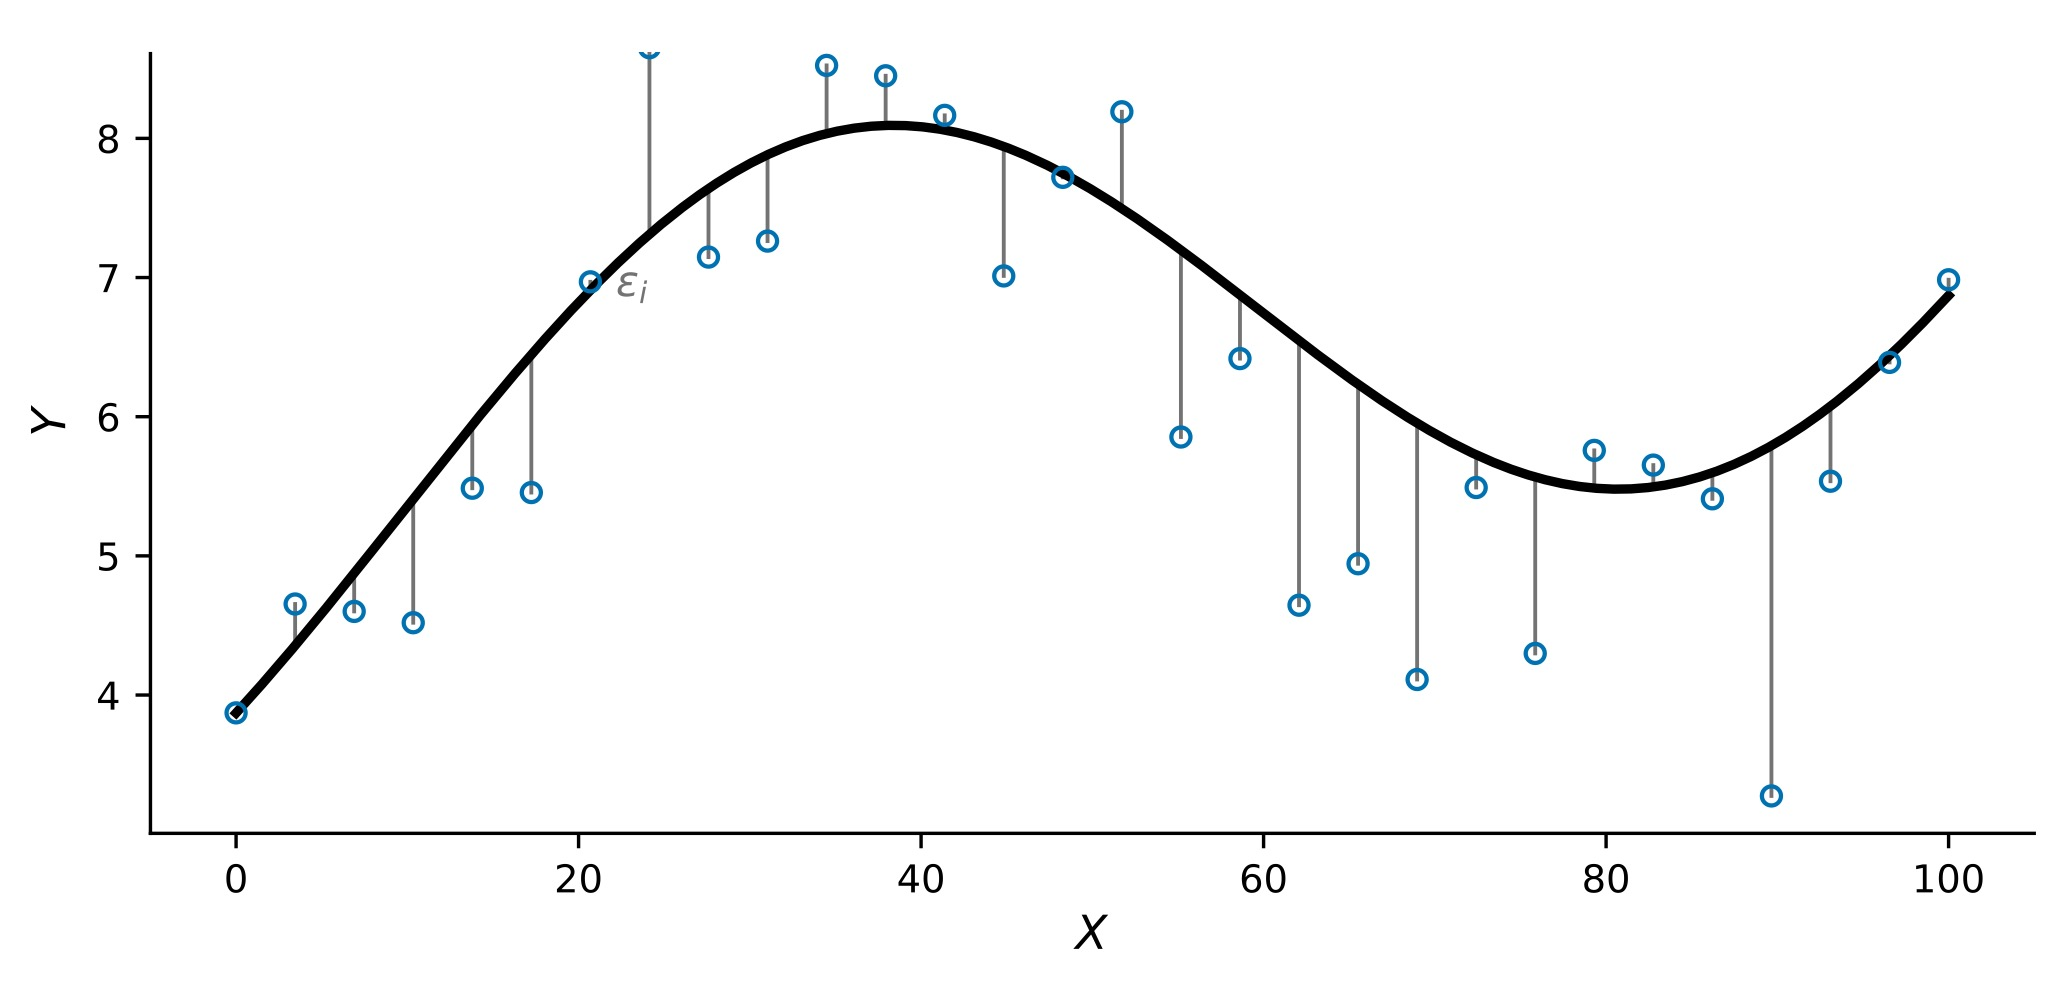
\includegraphics[width=0.75\linewidth]{img/regmodelgraph.JPG}
\end{figure}

\vspace{-1cm}
\begin{itemize}
    \item The black curve is $f(X) = \E [Y \mid X=x]$, the systematic relationship.
    \item The vertical segments are $\varepsilon_i=y_i-f(x_i)$, the unsystematic noise terms.
    \item Gien $X=x$, the observations vary around $f(x)$ with mean-zero noise and variance $\sigma^2$.
    \item \textbf{We never observe $f$ directly but rather the data scattered around it.}
\end{itemize}

\subsection{Goals of Learning}
Knowing $f$ is useful for two quite different reasons.
\begin{definition}[Prediction]\leavevmode \\
We want to \textit{predict} the response $Y$ from observed predictors $X$. We use
\begin{equation*}
    \hat{Y}:=\hat{f}(X)
\end{equation*}
where what matters is how accurately $\hat{f}(X)$ predicts $Y$; the form of $\hat{f}$ itself may be unimportant.
\end{definition}

\begin{definition}[Inference]\leavevmode \\
We want to \textit{understand} how the response $Y$ depends on the predictors $X$. We use
\begin{equation*}
    \hat{f}
\end{equation*}
to learn which predictors matter, in which direction, and how strongly. What matters is what $\hat{f}$ tells us about the relationship between $X$ and $Y$.
\end{definition}

\begin{table}[H]
\centering
\begin{tabular}{@{}l p{3.5cm} l@{}}
\toprule
 & Prediction & Inference\\
\midrule
main goal: & predict $Y$ accurately & understand how $Y$ depends on $X$\\
what matters: & $\hat{f}(x)$ is accurate & the structure of $\hat{f}$ is interpretable\\
complexity: & can be useful & can make interpretation harder\\
\botrule
\end{tabular}
\end{table}

\section{Evaluating Model Performance}
We observe a training set $\mathcal{D}=\{(x_1,y_1),\dots,(x_n,y_n)\}$ where $y_i=f(x_i)+\varepsilon_i$. A \textbf{statistical learning method} uses these data to construct an estimate of $f$: $\mathcal{D}\longmapsto \hat{f}_{\mathcal{D}}$. Because $\hat{f}$ is constructed from the data, different training samples will generally produce different fitted functions:$\mathcal{D}_1\longmapsto \hat{f}_{\mathcal{D}_1}$, $\mathcal{D}_2\longmapsto \hat{f}_{\mathcal{D}_2}$, $\dots$.

\subsection{Measuring Accuracy}


Suppose $\fhat$ has been fitted using the training data $\mathcal{D}$. Consider a new observation $(X_0,Y_0)$, drawn from the same population but not used to fit $\fhat$.

\begin{definition}[Mean Squared Prediction Error]\leavevmode \\
The mean squared prediction error (MSPE) of the fitted function $\fhat$ is
\begin{equation*}
    \E\big[\{Y_0-\fhat(X_0)^2\} \mid \mathcal{D} \big]
\end{equation*}
\end{definition}

The expectation averages over new observations $(X_0,Y_0)$, while the fitted function $\fhat$ is held fixed (by conditioning on the data $\data$). A good fitted model predicts new observations accurately, i.e. has small MSPE.

The MSPE is a population quantity and is generally unknown. Two sample quantities are useful: training MSE to measure fit and test MSE to measure prediction.
\begin{definition}[Training MSE] \leavevmode \\
Measures the fit to the \textbf{training data}, using the observations that were used to fit $\fhat$,
\begin{equation*}
     \text{MSE}_\text{train}=\frac{1}{n}\sum_{i=1}^{n}\{y_i-\fhat(x_i)\}^2
\end{equation*}
\end{definition}

\begin{definition}[Test MSE] \leavevmode \\
Estimates prediction error on \textbf{new data}, using new observations $(x_1^0,y_1^0),\dots,(x_m^0,y_m^0)$ not used to fit $\fhat$,
\begin{equation*}
     \text{MSE}_\text{test}=\frac{1}{m}\sum_{j=1}^{m}\{y_j^0-\fhat(x_j^0)\}^2
\end{equation*}
\end{definition}

\subsection{Model Complexity and Overfitting}
Different learning methods allow fitted functions of different complexity. For example, consider polynomials of increasing degree:
\begin{equation*}
    \mathcal{F}_1\subset \mathcal{F}_2\subset \mathcal{F}_3\subset\dots, \quad \mathcal{F}_d=\{\beta_0+\beta_1x+\dots+\beta_dx^d\}
\end{equation*}

A larger class is \textbf{more flexible}: it allows $\fhat$ to take a wider variety of shapes. \textit{Lower} flexibility would imply straighter lines while \textit{higher} flexibility increases the complexity of the curves. 

Greater flexibility makes it easier to fit the training data closely since as flexibility increases, we expect the fitted function to follow the training observations more closely. Hence, the training MSE should decrease. But the quantity we care about is the prediction error on new observations: \textbf{Does a smaller training MSE imply a smaller test MSE?}

\subsubsection{Training Error versus Test Error}
To find out, we simulate data from a known regression function $f$. The left panel shows one training sample and three polynomial fits, where increasing flexibility lets the fitted curve follow the training data more closely. The right panel shows the training and test MSE as the flexibility increases. The horizontal dashed line is $\Var(\varepsilon)=\sigma^2$, the irreducible error.

\begin{enumerate}
    \item \textbf{$f$ is Non-Linear} \newline
    \begin{figure}[H]\vspace{-0.75cm}
        \centering
        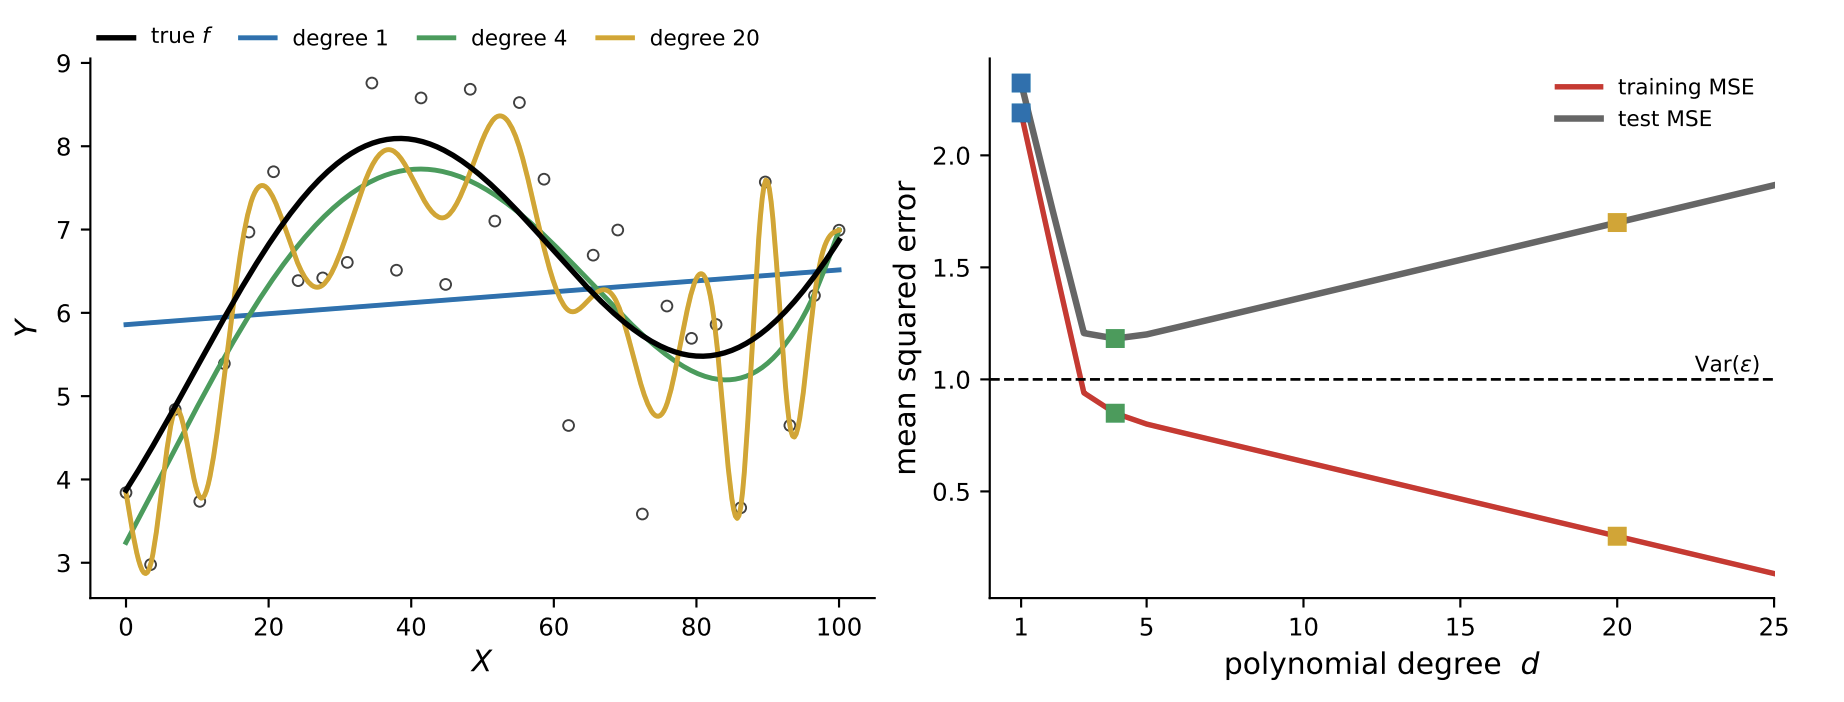
\includegraphics[width=0.75\linewidth]{img/s1nonlinear.png}
    \end{figure}\vspace{-0.5cm}
    \item \textbf{$f$ is Nearly Linear} \newline
    \begin{figure}[H]\vspace{-0.75cm}
        \centering
        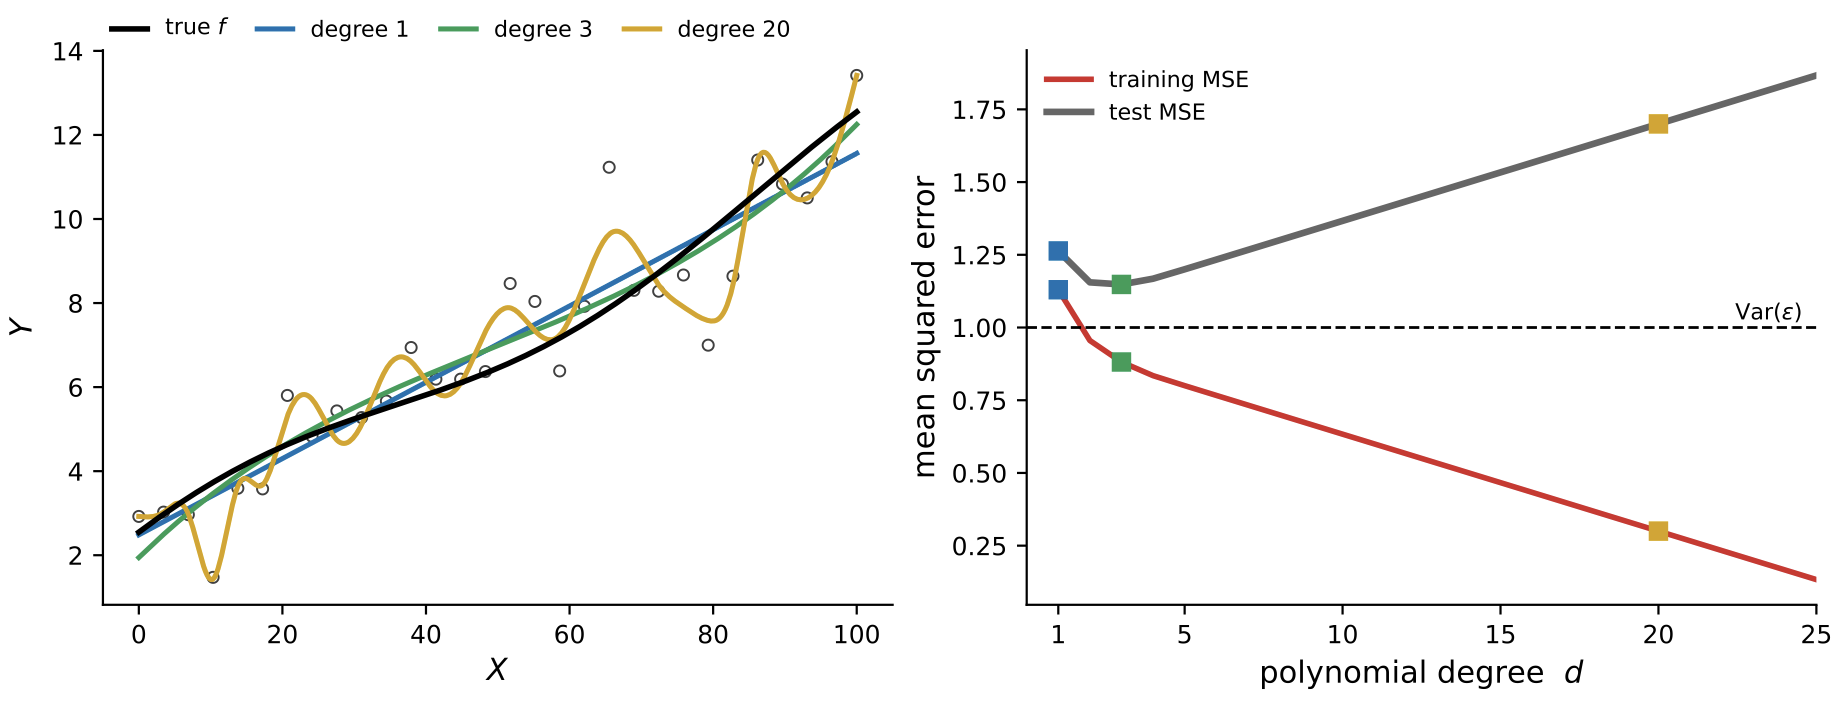
\includegraphics[width=0.75\linewidth]{img/s2nearlylinear.png}
    \end{figure}\vspace{-0.5cm}
    \item \textbf{$f$ is Highly Non-Linear} \newline
    \begin{figure}[H]\vspace{-0.75cm}
        \centering
        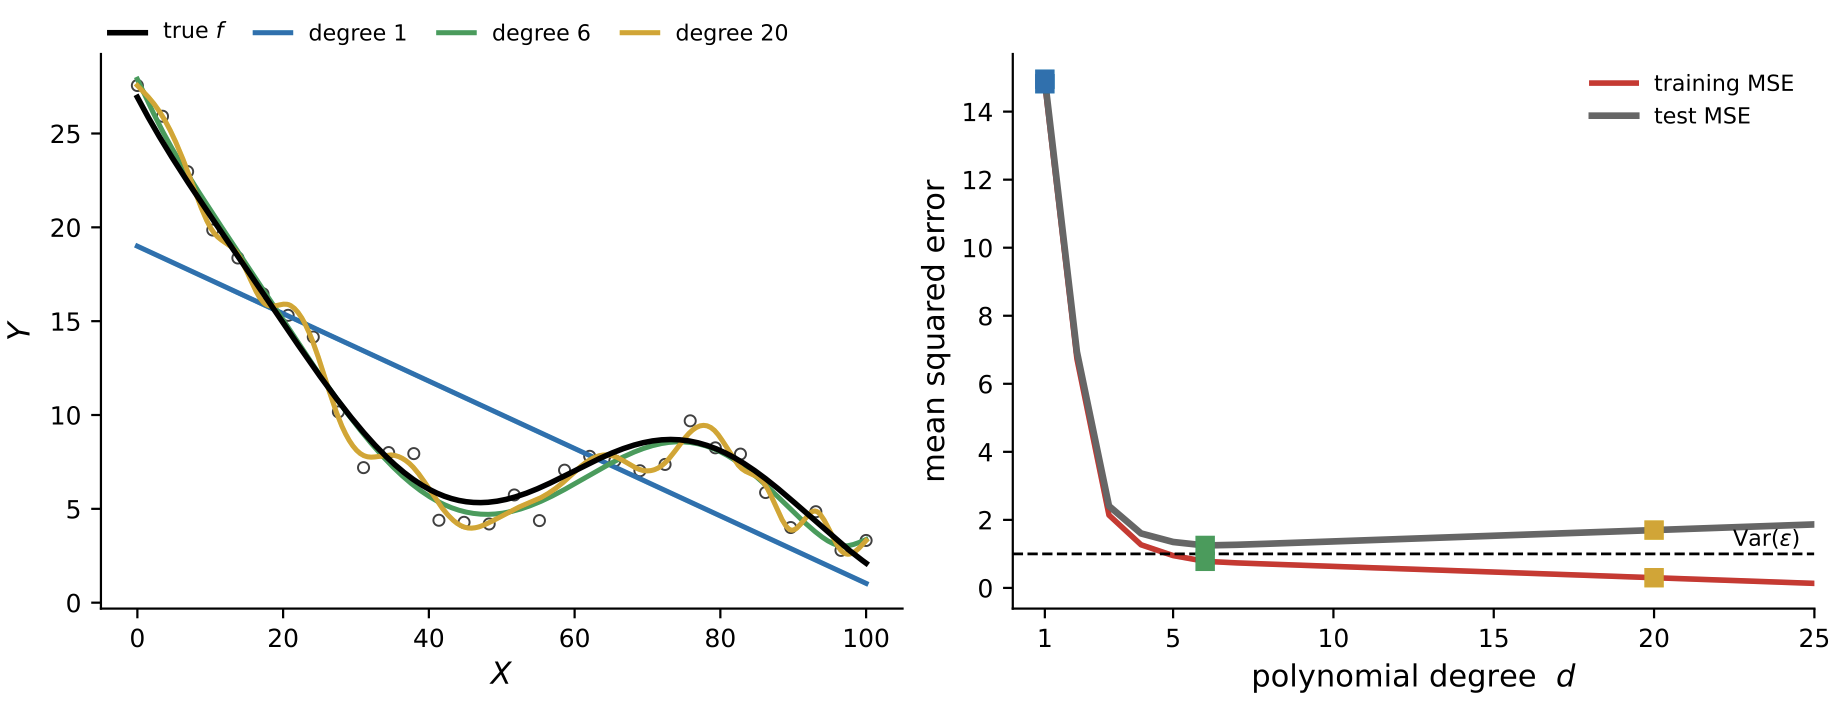
\includegraphics[width=0.75\linewidth]{img/s3highlynonlinear.png}
    \end{figure}\vspace{-0.5cm}
\end{enumerate}

The details differ across the three scenarious, but the qualitative message is stable:
\begin{itemize}
    \item Training MSE decreases as flexibility increases.
    \item Test MSE is typically U-shaped.
    \item The optimal flexibility depends on the unknown true function $f$.
    \item Training MSE therefore cannot be trusted to choose flexibility: it tends to prefer models that are too flexible.
\end{itemize}

\subsubsection{Overfitting}

\begin{definition}[Overfitting]
    Overfitting occurs when increasing flexibility improves fit to the training data but worsens prediction on new data.
\end{definition}
Overfitting is seen on the right-hand side of the U-shaped test-error curve. The mechanism is already visible in the regression model:

\begin{equation*}
    y_i=f(x_i)+\varepsilon_i
\end{equation*}
where $f(x_i)$ is the signal and $\varepsilon_i$ is the noise. A very flexible method adapts to both the signal and the sample-specific noise which does not repeat in a new sample. Overfitting means fitting features of the training data that do not generalise.

\subsection{Optimal Predictors and Bias-Variance Trade-off}
Suppose we could choose \textit{any} function $g$ to predict $Y$ from $X$. Under squared-error loss, its mean squared prediction error is
\begin{equation*}
    \E \big[\{Y-g(X)\}^2\big]
\end{equation*}

\begin{theorem}[Error Decomposition]\label{thm:errordecomp} \leavevmode \\
    Suppose
    \begin{equation*}
        Y=f(X)+\varepsilon, \quad \E[\varepsilon \mid X]=0, \quad \Var(\varepsilon \mid X)=\sigma^2
    \end{equation*}
    Then, for any predictor $g(X)$,
    \begin{equation*}
        \E \big[\{Y-g(X)\}^2\big] = \E \big[\{f(X)-g(X)\}^2\big] + \sigma^2
    \end{equation*}
\end{theorem}

Since $\E \big[\{f(X)-g(X)\}^2\big] \geq 0$, the mean squared predictor error is minimise by setting $g(X)$ equal to
\begin{equation*}
    f(X)=\E[Y \mid X]
\end{equation*}
Therefore, the regression function is the best possible predictor of $Y$ under squared error.

\subsubsection{Reducible and Irreducible Error}
Hold the fitted function $\fhat$ fixed and consider prediction on a new observation. By theorem (\ref{thm:sqerror}),
\begin{equation*}
    \E \Big[\{Y_0-\fhat(X_0)\}^2 \Big| \data\Big]
    =
    \E \Big[\{f(X_0)-\fhat(X_0)\}^2 \Big| \data\Big] + \sigma^2
\end{equation*}

\begin{definition}[Reducible Error]\leavevmode\\
    Our fitted function $\fhat$ differs from the true regression function $f$. Better estimation of $f$ can reduce this part.
\end{definition}

\begin{definition}[Irreducible Error]\leavevmode\\
    Even if $\fhat = f$, the response still varies around $f(X)$ because of the noise $\varepsilon$. No prediction method can remove this part.
\end{definition}

With the learning method fixed, $\fhat(x_0)$ is random because the training data are random. 
\begin{equation*}
    \data \longmapsto \fhat_\data \longmapsto \fhat_\data(x_0)
\end{equation*}

If we repeatedly collect new training sampples and refit the model, we obtain different predictions at the same point $x_0$:
\begin{equation*}
    \fhat_{\data_{1}}(x_0), \quad \fhat_{\data_{2}}(x_0), \quad \fhat_{\data_{3}}(x_0), \quad \dots
\end{equation*}

Thus, $\E[\fhat(x_0)$ and $\Var(\fhat(x_0)$ refer to repeated training samples. Estimation introduces a second source of randomness: the training sample itself.

\begin{figure}[H]
    \centering
    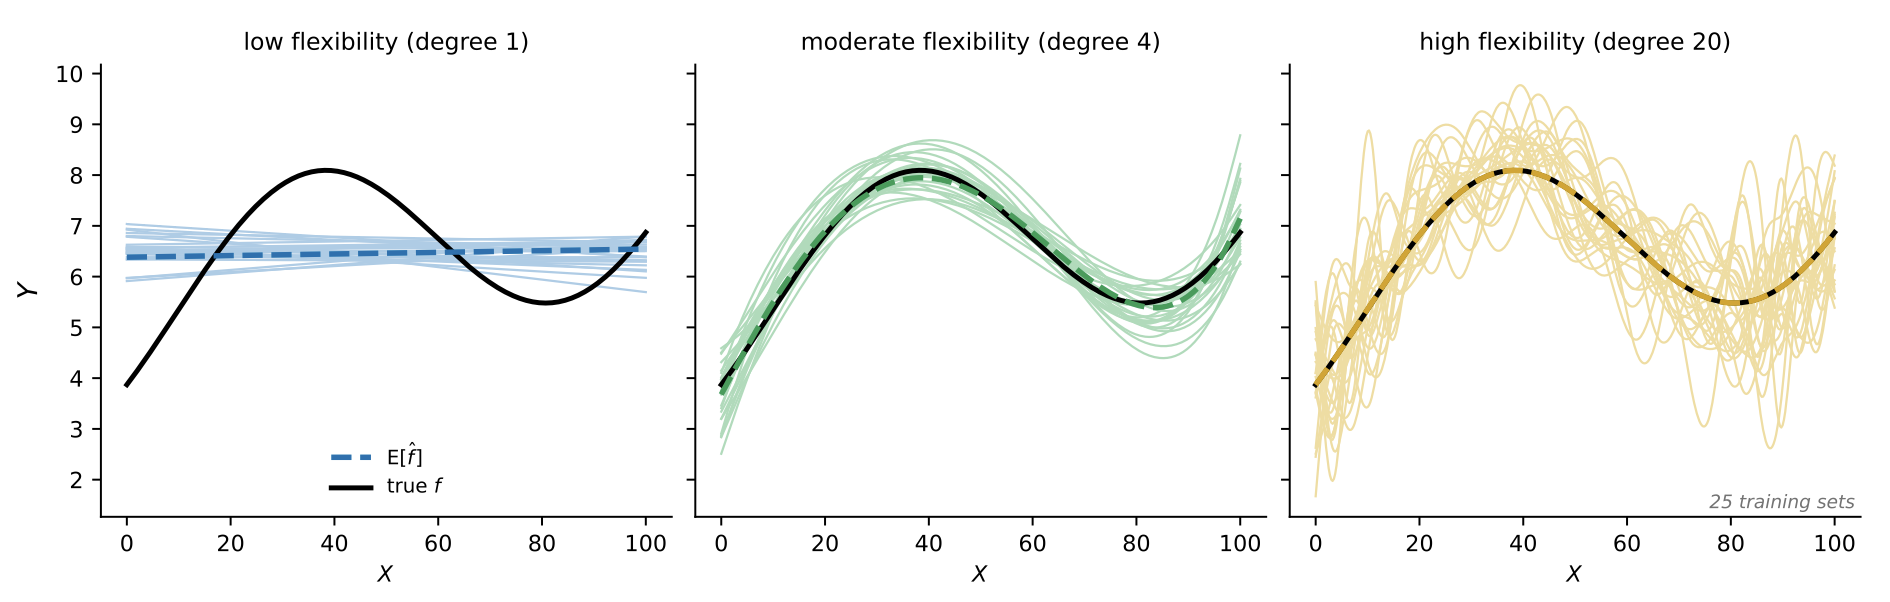
\includegraphics[width=0.8\linewidth]{img/flexibilityaveragefit.png}
\end{figure}\vspace{-0.5cm}
Each thin curve is fitted from different training sets generated from the same population. The dashed curve is the average fit $\E[\fhat]$; the black curve is the truth $f$. We see two entirely different things can go wrong at fixed point $x_0$.

\begin{definition}[Bias]\leavevmode\\
Measures systematic error
    \begin{equation*}
        \Bias (\fhat(x_0)) := \E[\fhat(x_0)]-f(x_0)
    \end{equation*}
\end{definition}

\textbf{Systematically wrong:} The method aims at the wrong place where $\E[\fhat(x_0)] \neq f(x_0)$. The fitted curves agree with one another but systematically miss $f$.

\begin{definition}[Variance]\leavevmode\\
Measures sample-to-sample instability
    \begin{equation*}
        \Var(\fhat(x_0)):= \E \Big[\big\{\fhat(x_0)-\E[\fhat(x_0)]\big\}^2\Big]
    \end{equation*}
\end{definition}

\textbf{Unstable:} The method changes substantially from one training sample to another. The fits are close to $f$ on average but individual fits vary widely.

Low flexibility tends to produce more bias and less variance while high flexibility tends to produce less bias and more variance.

\subsubsection{Mean Squared Error Decomposition}
Fix a test point $x_0$ and consider a new response
\begin{equation*}
    Y_0=f(x_0)+\varepsilon_0, \quad \E[\varepsilon_0]=0, \quad \Var(\varepsilon_0)=\sigma^2
\end{equation*}
The training data used to construct $\fhat$ are independent of the new noise $\varepsilon_0$. We study the \textbf{expected test error} at $x_0$,
\begin{equation*}
    \E \big[(Y_0-\fhat(x_0))^2\big]
\end{equation*}
where the expectation averages over both (1) the random training data that determine $\fhat$, and (2) the new response $Y_0$.

\begin{theorem}[Mean Squared Error Decomposition]\leavevmode\\
    For a fixed test point $x_0$,
    \begin{equation*}
        \E\big[(Y_0-\fhat(x_0))^2\big]=\sigma^2+\Bias(\fhat(x_0))^2 + \Var(\fhat(x_0))
    \end{equation*}
\end{theorem}

\begin{itemize}
    \item \textbf{Irreducible noise} ($\sigma^2$): randomness in $Y_0$ that no method can predict
    \item \textbf{Squared Bias} ($\Bias(\fhat(x_0))^2$): systematic error of the learning model
    \item \textbf{Variance} ($\Var(\fhat(x_0))$): instability cause by estimating $f$ from a random finite sample
\end{itemize}

\begin{table}[H]\vspace{-0.5cm}
\centering
\begin{tabular}{@{}l p{5cm} l@{}}
\toprule
Term & What it measures & How can it change?\\
\midrule
$\sigma^2$ & noise in $Y$ given $X$ & cannot be reduced\\
$\Bias(\fhat(x_0))^2$ & systematic error & typically falls with flexibility\\
$\Var(\fhat(x_0))$ & sample-to-sample instability & typically rises with flexibility\\
\botrule
\end{tabular}
\end{table}

Thus, increasing flexibility typically has opposite effects:
\begin{equation*}
    \text{more flexibility} \Longrightarrow 
    \begin{cases} 
    \text{lower bias,} \\ 
    \text{higher variance}
    \end{cases}
\end{equation*}

\begin{figure}[H]\vspace{-0.75pt}
    \centering
    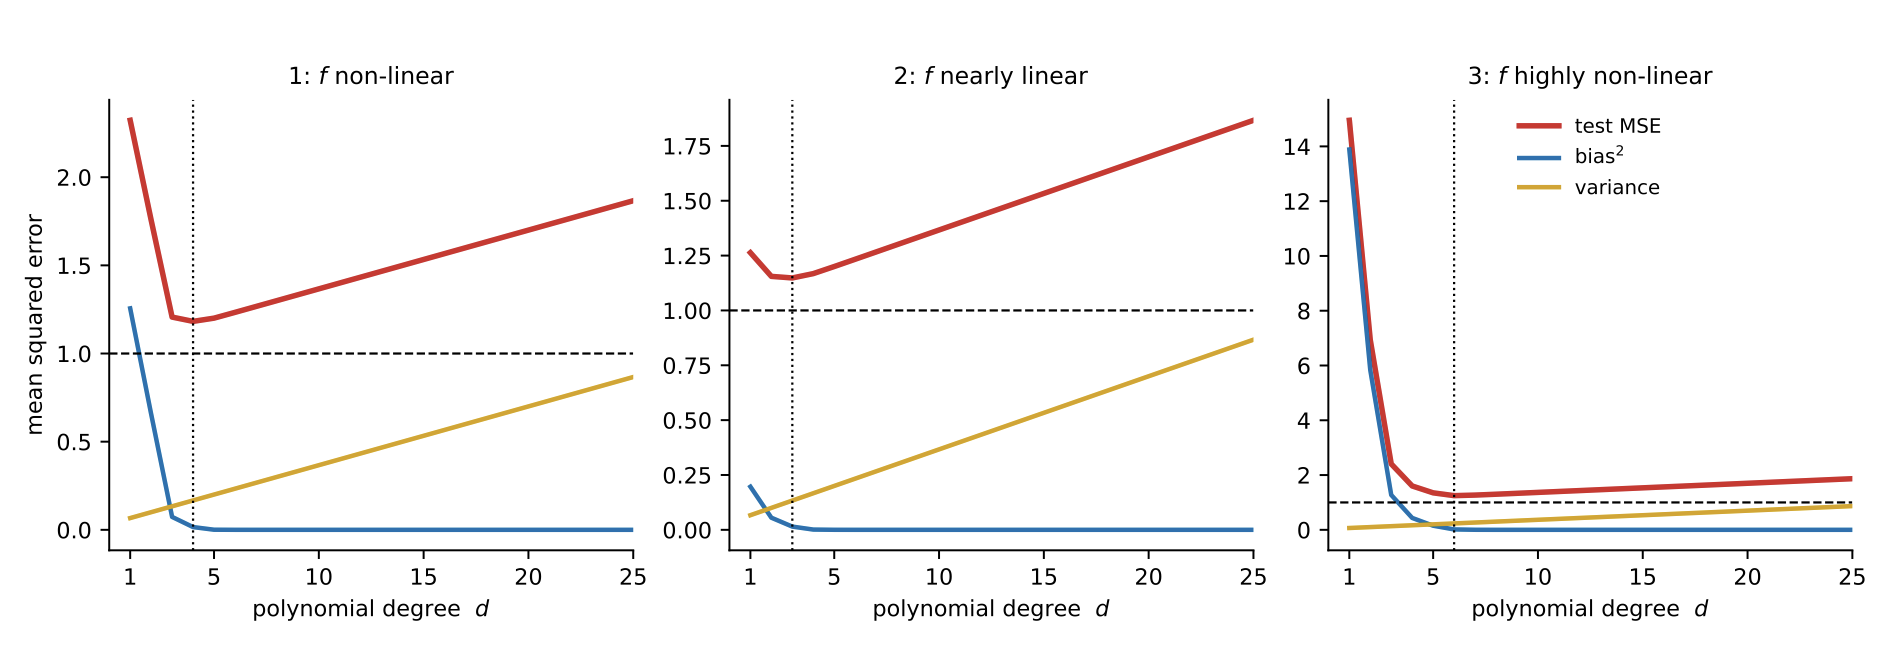
\includegraphics[width=0.75\linewidth]{img/flexibility3.png}
\end{figure}\vspace{-0.7pt}
We see that in every panel, squared bias (blue) decreases and variance (yellow) increases with flexibility. Their sum, plus the constant $\sigma^2$, produces the test MSE (red) curve.

\begin{figure}[H]\vspace{-0.75pt}
    \centering
    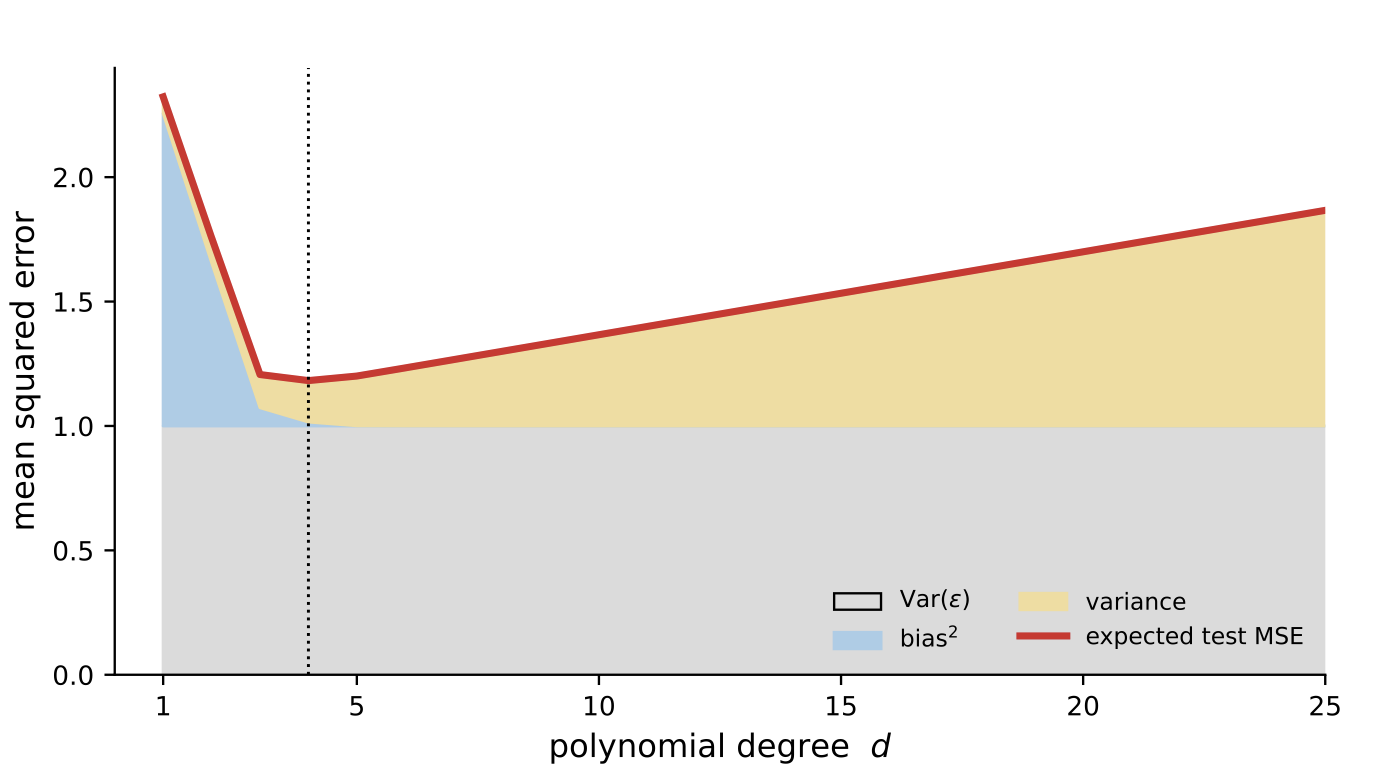
\includegraphics[width=0.6\linewidth]{img/flexibilitystacked.png}
\end{figure}\vspace{-0.75pt}
Stacking the lines, we see that:
\begin{itemize}
    \item The grey floor $\sigma^2$ is there whatever we do
    \item Squared bias (blue) shrinks as we move right; variance (yellow) grows
    \item The optimum is where their total is the smallest (red)
\end{itemize}

The opposite dependence of bias and variance on flexibility is the \textbf{bias-variance trade-off}. At first, increasing flexibility may reduce squared bias by more than it increases variance. Eventually, the increase in variance dominates.

\begin{table}[H]\vspace{-0.5cm}
\centering
\begin{tabular}{ccc}
\toprule
Low flexibility & Moderate flexibility & High flexibility\\
\midrule
high bias & lower bias & low bias\\
low variance & moderate variance & high variance\\
underfitting & good prediction & overfitting\\
\botrule
\end{tabular}
\end{table}\vspace{-0.5cm}

The optimal flexibility depends on the unknown $f$, the noise level, and the amount of data available.



\providecommand{\E}{\operatorname{E}}
\providecommand{\Var}{\operatorname{Var}}
\providecommand{\fhat}{\hat{f}}
\providecommand{\data}{\mathcal{D}}
\providecommand{\Bias}{\operatorname{Bias}}
\providecommand{\Cov}{\operatorname{Cov}}
\providecommand{\thetahat}{\hat\theta}
\providecommand{\betahat}{\hat{\bm\beta}}


\chapter{Linear Regression and Extensions}
\label{ch:topic2}

\section{Formulation and Estimation of Linear Least Squares}

\subsection{The Population Problem and Empirical Risk Minimization}

\subsubsection{The Population Problem}
Let
\begin{equation*}
    X=(X_1,\dots,X_d)^\top, \quad \widetilde{X}=(1,X^\top)^\top \in \mathbb{R}^p, \quad p=d+1
\end{equation*}

and suppose
\begin{equation*}
    \E[Y^2] < \infty, \quad \E[\lVert X \rVert_2^2]<\infty
\end{equation*}

We restrict attention to linear predictors
\begin{equation*}
    g_\beta=\widetilde{X}^\top\bm\beta, \quad \bm{\beta}=(\beta_0,\beta_1,\dots,\beta_d)^\top \in \mathbb{R}^p
\end{equation*}

and measure their prediction error by
\begin{equation*}
    L(\bm\beta):=\E \Big[\{Y-\widetilde{X}^\top\bm\beta\}^2\Big]
\end{equation*}

\begin{definition}[Best Linear Predictor] \leavevmode \\
    The best linear predictor is
    \begin{equation*}
        g^*(X)=\widetilde{X}^\top\bm\beta^*, \quad \bm\beta^*\in \arg \min_{\bm\beta\in\mathbb{R}^p}L(\bm\beta)
    \end{equation*}
\end{definition}

\subsubsection{Optimal Conditions}
Recall the loss function:
\begin{equation*}
    L(\bm\beta) = \E \Big[\{Y-\widetilde{X}^\top\bm\beta\}^2\Big]
\end{equation*}

\textbf{First-order condition:} Taking the gradient with respect to $\bm\beta$ gives:
\begin{equation*}
    \nabla L(\bm\beta) = -2\E \Big[\widetilde{X}\{Y-\widetilde{X}^\top\bm\beta\}\Big]
\end{equation*} 

Hence, setting the gradient to zero at the optimal weights $\bm\beta^*$, we have:
\begin{equation*}
    \E \Big[\widetilde{X}\{Y-\widetilde{X}^\top\bm\beta^*\}\Big] = 0
\end{equation*}

\textbf{Second-order condition:} The Hessian matrix is:
\begin{equation*}
    \nabla^2 L(\bm\beta) = 2\E \big[\widetilde{X}\widetilde{X}^\top\big]
\end{equation*}

and, for every vector $a \in \mathbb{R}^p$:
\begin{equation*}
    a^\top \nabla^2 L(\bm\beta) a = 2\E \big[(a^\top \widetilde{X})^2\big] \geq 0
\end{equation*}

Thus, $L$ is convex. Hence, every solution $\bm\beta^*$ is a global minimizer.

\subsection*{Solving the First-Order Conditions \& The Solution}

We begin by splitting the optimal weights vector into the intercept $\beta_0^*$ and the slope coefficients $\bm\beta_{-0}^* \in \mathbb{R}^d$:
\begin{equation*}
    \bm\beta^* = (\beta_0^*, \bm\beta_{-0}^{*\top})^\top
\end{equation*}

Expanding the first-order condition from the previous step yields two separate equations:
\begin{align*}
    \E[Y - \beta_0^* - \bm\beta_{-0}^{*\top}X] &= 0 \\
    \E[X\{Y - \beta_0^* - \bm\beta_{-0}^{*\top}X\}] &= 0
\end{align*}

The first equation allows us to easily isolate the intercept:
\begin{equation*}
    \beta_0^* = \E[Y] - \bm\beta_{-0}^{*\top}\E[X]
\end{equation*}

We then substitute this intercept back into the second equation:
\begin{equation*}
    0 = \E\big[X\{Y - \E[Y]\}\big] - \E\big[X(X - \E[X])^\top\big]\bm\beta_{-0}^*
\end{equation*}

Notice that the two expectations in this equation are exactly the population covariance quantities. Because $\E[Y - \E[Y]] = 0$ and $\E[X - \E[X]] = 0$, we can rewrite them as:
\begin{align*}
    \E\big[X\{Y - \E[Y]\}\big] &= \E\big[(X - \E[X])\{Y - \E[Y]\}\big] = \Cov(X,Y) \\
    \E\big[X(X - \E[X])^\top\big] &= \E\big[(X - \E[X])(X - \E[X])^\top\big] = \Cov(X)
\end{align*}

Define $\Sigma_{XX} := \Cov(X)$ and $\Sigma_{XY} := \Cov(X,Y)$. The slope coefficients must therefore satisfy:
\begin{equation*}
    \Sigma_{XX}\bm\beta_{-0}^* = \Sigma_{XY}
\end{equation*}

Thus, if the covariance matrix $\Sigma_{XX}$ is invertible, we arrive at the final unique solution for the best linear predictor:
\begin{equation*}
    \bm\beta_{-0}^* = \Sigma_{XX}^{-1}\Sigma_{XY}, \quad \beta_0^* = \E[Y] - \bm\beta_{-0}^{*\top}\E[X]
\end{equation*}

\subsubsection{First-Order Conditions}
Define the population residual
\begin{equation*}
    \varepsilon^*:=Y-g^*(X)
\end{equation*}

The first-order conditions become
\begin{align*}
    \E[\varepsilon^*] &= 0, \\
    \E[X_j\varepsilon^*] &=0, \quad j=1,\dots,d.
\end{align*}

Therefore,
\begin{align*}
    \Cov(X_j,\varepsilon^*) &= \E[X_j\varepsilon^*]-\E[X_j]E[\varepsilon^*] \\
    &= 0, \quad j=1,\dots,d.
\end{align*}

The residual from the best linear predictor is \textbf{uncorrelated} with every predictor.

\subsubsection{Non-linear Regression Function}
Under the regression model,
\begin{equation*}
    f(X)=\E[Y \mid X]
\end{equation*}

is the best predictor among all functions of $X$, whereas
\begin{equation*}
    g^*(X)=\beta_0^*+{\bm\beta^{\bm*}}^{\top}X
\end{equation*}

is the best predictor among linear functions. If $f$ is not linear, these generally differ $g^*(X) \neq f(X)$. From Theorem \ref{thm:errordecomp}, the approximation error $\E \big[\{f(X)-g^*(X)\}^2\big]$ is 0 when $f(X)=g^*(X)$ almost surely. Restricting the model class to linear functions can create approximation error.

\subsubsection{From the Population to the Sample}
\begin{theorem}[Weak Law of Large Numbers]\leavevmode\\
    If $W_1,\dots,W_n$ are i.i.d. with
    \begin{equation*}
        \E[W_i]=\mu, \quad \Var(W_i)<\infty,
    \end{equation*}
    then, for every $\epsilon > 0$,
    \begin{equation*}
        \mathbb{P}\bigg(\bigg|\frac{1}{n}\sum_{i=1}^{n}W_i-\mu\bigg|>\epsilon\bigg)\longrightarrow 0.
    \end{equation*}
\end{theorem}

In order words, as the sample size grows, the sample average converges to the population average. For example,
\begin{equation*}
    \frac{1}{n}\sum_{i=1}^{n}x_iy_i\approx\E[XY], \quad
    \frac{1}{n}\sum_{i=1}^{n}x_ix_i^\top\approx\E[XX^\top]
\end{equation*}

If the population distribution were known, we would minimise
\begin{equation*}
    L(\beta_0,\bm\beta)=\E\Big[\{Y-\beta_0-\bm\beta^\top X\}^2\Big]
\end{equation*}

But with i.i.d. observations $(x_i,y_i)_{i=1}^{n}$, replace the population average by its sample analogue:
\begin{equation*}
    L_n(\beta_0,\bm\beta)=\frac{1}{n}\sum_{i=1}^{n}\{y_i-\beta_0-\bm\beta^\top x_i\}^2
\end{equation*}

Then solve the sample (a.k.a. empirical) optimisation problem: \textbf{empirical risk minimisation}
\begin{equation*}
    (\widehat{\beta}_0,\widehat{\bm\beta})\in\arg \min_{\beta_0,\bm\beta}L_n(\beta_0,\bm\beta)
\end{equation*}

\subsubsection{Solving the Sample Problem: One Predictor}

For a single predictor ($d=1$), the empirical loss function is:
\begin{equation*}
    L_n(\beta_0, \beta_1) = \frac{1}{n}\sum_{i=1}^n (y_i - \beta_0 - \beta_1 x_i)^2
\end{equation*}

\textbf{First-order condition:}
Setting the partial derivatives to zero:
\begin{align*}
    \frac{\partial L_n}{\partial \beta_0} &= -\frac{2}{n}\sum_{i=1}^n (y_i - \beta_0 - \beta_1 x_i) = 0 \\
    \frac{\partial L_n}{\partial \beta_1} &= -\frac{2}{n}\sum_{i=1}^n x_i(y_i - \beta_0 - \beta_1 x_i) = 0
\end{align*}

Thus, any minimizer $(\hat{\beta}_0, \hat{\beta}_1)$ must satisfy:
\begin{align*}
    \sum_{i=1}^n (y_i - \hat{\beta}_0 - \hat{\beta}_1 x_i) &= 0 \\
    \sum_{i=1}^n x_i(y_i - \hat{\beta}_0 - \hat{\beta}_1 x_i) &= 0
\end{align*}

\textbf{Second-order condition:} The Hessian matrix is:
\begin{equation*}
    \nabla^2 L_n(\beta_0, \beta_1) = \frac{2}{n}
    \begin{pmatrix}
        n & \sum_{i=1}^n x_i \\
        \sum_{i=1}^n x_i & \sum_{i=1}^n x_i^2
    \end{pmatrix}
\end{equation*}

For any vector $(a, b) \in \mathbb{R}^2$:
\begin{equation*}
    (a, b) \nabla^2 L_n(\beta_0, \beta_1) 
    \begin{pmatrix} 
        a \\ 
        b 
    \end{pmatrix} 
    = \frac{2}{n}\sum_{i=1}^n (a + b x_i)^2 \geq 0
\end{equation*}

Hence, $L_n$ is convex, and $(\hat{\beta}_0, \hat{\beta}_1)$ is a global minimizer.

\textbf{Solving the equations:} The first normal equation gives:
\begin{equation*}
    \hat{\beta}_0 = \bar{y} - \hat{\beta}_1 \bar{x}, \quad \text{where } \bar{x} = \frac{1}{n}\sum_{i=1}^n x_i, \quad \bar{y} = \frac{1}{n}\sum_{i=1}^n y_i
\end{equation*}

Substituting this into the second equation:
\begin{equation*}
    \hat{\beta}_1 = \frac{\sum_{i=1}^n (x_i - \bar{x})(y_i - \bar{y})}{\sum_{i=1}^n (x_i - \bar{x})^2}
\end{equation*}

\begin{figure}[H]
    \centering
    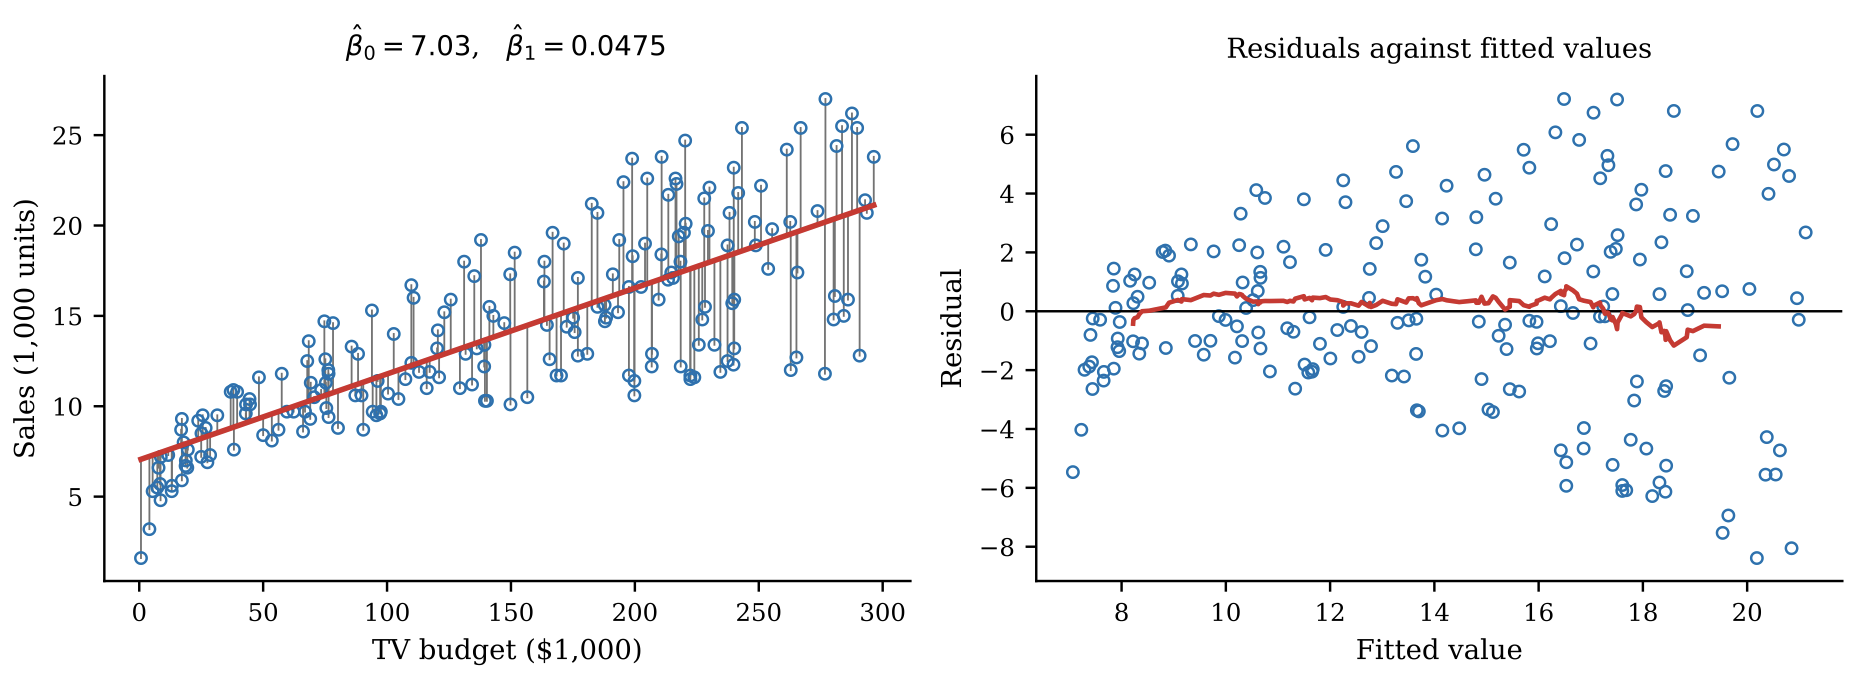
\includegraphics[width=0.8\linewidth]{img/residuals.png}
\end{figure}

\begin{itemize}
    \item \textbf{Left:} the least squares line minimised the total squared length of the grey segments/
    \item \textbf{Right:} the residuals $e_i=y_i-\hat{y}_i$ against the fitted values $\hat{y}_i$. By construction, they average to zero and are orthogonal to the fitted values: $\sum_{i=1}^ne_i=0 \Rightarrow \bar{e}=0$
\end{itemize}

\subsection{Matrix Foundations and Least Squares Solution}

\subsubsection{Matrix Toolbox}
Let $\bm{u}, \bm{v} \in \mathbb{R}^n$.

\begin{definition}[Inner Product]\leavevmode\\
    The \textbf{Euclidean inner product} of $\bm{u}$ and $\bm{v}$ is
    \begin{equation*}
        \langle\bm{u},\bm{v}\rangle:=\bm{u}^\top \bm{v} = \sum_{i=1}^{n}u_i v_i
    \end{equation*}
\end{definition}

\begin{definition}[Euclidean Norm]\leavevmode\\
    The \textbf{Euclidean norm} of $\bm{v}$ is
    \begin{equation*}
        \lVert \bm{v} \rVert_2:= \sqrt{\bm{v}^\top\bm{v}} = \Bigg( \sum_{i=1}^{n}{v_i^2}\Bigg)^{1/2}
    \end{equation*}

    Hence,
    \begin{equation*}
        \lVert \bm{v} \rVert_2^2 = \bm{v}^\top \bm{v}
    \end{equation*}

    (The Euclidean norm measures the length of a vector.)
\end{definition}

\noindent
Let $\bm{A} \in \mathbb{R}^{n \times p}$, with columns $\bm{a}_1,\dots,\bm{a}_p \in \mathbb{R}^n$.

\begin{definition}[Column Space and Rank] \leavevmode\\
    The \textbf{column space} and \textbf{rank} of $\bm{A}$ are
    \begin{equation*}
        \operatorname{col}(\bm{A}) = \operatorname{span}\{\bm{a}_1,\dots,\bm{a}_p\}, \quad
        \operatorname{rank}(\bm{A})=\operatorname{dim}\{\operatorname{col}(\bm{A})\}.
    \end{equation*}

    Thus, $\operatorname{rank}(\bm{A}) = p$ exactly when the columns of $\bm{A}$ are linearly independent.
\end{definition}

\begin{definition}[Orthogonality]
    Two vectors are \textbf{orthogonal} if
    \begin{equation*}
        \bm{u}\perp \bm{v} \quad 
        \Longleftrightarrow \quad
        \bm{u}^{\top}\bm{v}=0
    \end{equation*}

    Moreover,
    \begin{equation*}
        \bm{v} \perp \operatorname{col}(\bm{A}) \quad
        \Longleftrightarrow \quad
        \bm{A}^\top\bm{v}=0 \quad
        \Longleftrightarrow \quad
        \bm{a}_j^\top \bm{v} = 0, \quad j=1,\dots,p.
    \end{equation*}
\end{definition}

\noindent
Let $\bm{A} \in \mathbb{R}^{p \times p}$ be symmetric.

\begin{table}[H]
\centering
\begin{tabular}{lll}
\toprule
\textbf{Property} & \textbf{Notation} & \textbf{Definition} \\
\midrule
positive definite & $\bm{A} \succ  0$ & $\bm{v}^\top \bm{A}\bm{v} > 0$ for all $\bm{v} \neq \bm{0}$ \\
positive semidefinite & $\bm{A} \succeq 0$ & $\bm{v}^\top \bm{A}\bm{v} \geq 0$ for all $\bm{v}$ \\
negative definite & $\bm{A} \prec 0$ & $\bm{v}^\top \bm{A}\bm{v} < 0$ for all $\bm{v} \neq \bm{0}$ \\
negative semidefinite & $\bm{A} \preceq 0$ & $\bm{v}^\top \bm{A}\bm{v} \leq 0$ for all $\bm{v}$ \\
indefinite & & $\bm{v}^\top \bm{A}\bm{v}$ takes both signs\\
\botrule
\end{tabular}
\end{table}

For every $\bm{X} \in \mathbb{R}^{n \times p}$,
\begin{equation*}
    \bm{v}^\top \bm{X}^\top \bm{X}\bm{v} = (\bm{X}\bm{v})^\top (\bm{X}\bm{v}) = \lVert \bm{X}\bm{v} \rVert_2^2 \geq 0
\end{equation*}

so
\begin{equation*}
    \bm{X}^\top \bm{X} \succeq 0.
\end{equation*}

Moreover,
\begin{equation*}
    \bm{X}^\top \bm{X} \succ 0 \quad \Longleftrightarrow \quad \operatorname{rank}(\bm{X}) = p \quad \Longleftrightarrow \quad \bm{X}^\top \bm{X} \text{ is invertible.}
\end{equation*}

\begin{definition}[Trace]\leavevmode\\
    Let $\bm{A}, \bm{B} \in \mathbb{R}^{p \times p}$. The \textbf{trace} of $\bm{A}$ is the sum of its diagonal entries:
    \begin{equation*}
        \operatorname{tr}(\bm{A}) := \sum_{j=1}^p A_{jj}.
    \end{equation*}
    The trace is linear: $\operatorname{tr}(a\bm{A} + b\bm{B}) = a \operatorname{tr}(\bm{A}) + b \operatorname{tr}(\bm{B})$ for all $a, b \in \mathbb{R}$.
\end{definition}

\begin{theorem}[Cyclicity of the Trace]\leavevmode\\
    Let $\bm{A} \in \mathbb{R}^{p \times q}$, $\bm{B} \in \mathbb{R}^{q \times r}$, $\bm{C} \in \mathbb{R}^{r \times p}$. Then,
    \begin{equation*}
        \operatorname{tr}(\bm{A}\bm{B}\bm{C}) = \operatorname{tr}(\bm{B}\bm{C}\bm{A}) = \operatorname{tr}(\bm{C}\bm{A}\bm{B}).
    \end{equation*}
    More generally, factors inside a trace may be cyclically permuted whenever their products are well defined.

    \vspace{0.5em}
    \noindent
    \textbf{Trivial (but important) fact:} If $\bm{A} \in \mathbb{R}^{1 \times 1}$ (i.e. $\bm{A}$ is a scalar), then $\operatorname{tr}(\bm{A}) = \bm{A}$.
\end{theorem}

\subsubsection{Matrix Notation}

For observation $i$, write
\begin{equation*}
    X_i = (x_{i1}, \dots, x_{id})^\top \in \mathbb{R}^d
\end{equation*}

for its observed predictor vector. Collect the $n$ observations in the design matrix
\begin{equation*}
    X = \begin{pmatrix}
        1 & X_1^\top \\
        1 & X_2^\top \\
        \vdots & \vdots \\
        1 & X_n^\top
    \end{pmatrix} = \begin{pmatrix}
        1 & x_{11} & \cdots & x_{1d} \\
        1 & x_{21} & \cdots & x_{2d} \\
        \vdots & \vdots & \ddots & \vdots \\
        1 & x_{n1} & \cdots & x_{nd}
    \end{pmatrix} \in \mathbb{R}^{n \times p}, \quad p = d+1.
\end{equation*}

Define
\begin{equation*}
    y = (y_1, \dots, y_n)^\top, \quad \beta = (\beta_0, \beta_1, \dots, \beta_d)^\top.
\end{equation*}

Then
\begin{equation*}
    y = X\beta + \epsilon, \quad L_n(\beta) := \frac{1}{n} \lVert y - X\beta \rVert_2^2.
\end{equation*}

\subsection*{Solving the Least-Squares Problem}

The least-squares objective function in matrix notation is:
\begin{equation*}
    L_n(\bm\beta) = \frac{1}{n} \|y - X\bm\beta\|_2^2 = \frac{1}{n}(y - X\bm\beta)^\top (y - X\bm\beta)
\end{equation*}

\textbf{First-order condition:} Setting the gradient with respect to $\bm\beta$ to zero:
\begin{equation*}
    \nabla L_n(\bm\beta) = -\frac{2}{n} X^\top (y - X\bm\beta) = \mathbf{0}
\end{equation*}

This yields the \textbf{normal equations}:
\begin{equation*}
    X^\top X \hat{\bm\beta} = X^\top y
\end{equation*}

\textbf{Second-order condition:} The Hessian matrix is:
\begin{equation*}
    \nabla^2 L_n(\bm\beta) = \frac{2}{n} X^\top X
\end{equation*}

For any non-zero vector $v \in \mathbb{R}^p$:
\begin{equation*}
    v^\top \nabla^2 L_n(\bm\beta) v = \frac{2}{n} \|Xv\|_2^2 \geq 0
\end{equation*}

Thus, $L_n$ is convex. If $\text{rank}(X)=p$, then $X^\top X$ is invertible and the minimiser is unique:
\begin{equation*}
    \hat{\bm\beta} = (X^\top X)^{-1} X^\top y
\end{equation*}

Once $\hat{\bm\beta}$ has been computed, the vector of fitted values is
\begin{equation*}
    \hat{\bm{y}} :=   (\hat{y}_1,\dots,\hat{y}_n)^\top=X\hat{\bm\beta}= X(X^\top X)^{-1} X^\top y
\end{equation*}

\begin{definition}[Hat Matrix] \leavevmode\\
    The matrix
    \begin{equation*}
        H:=X(X^\top X)^{-1} X^\top
    \end{equation*}
    is called the hat matrix.
\end{definition}

Thus, the fitted values and residuals are
\begin{equation*}
    \hat{\bm{y}}=Hy, \quad \bm{e}:=\bm{y}-\hat{\bm{y}}=(I-H)\bm{y}
\end{equation*}

where $H$ maps the observed responses $\bm{y}$ to their fitted values $\hat{\bm{y}}$.


\section{Geometry, Projection, and Error Analysis}

\subsection{Orthogonality and Geometric Projection}

\subsubsection{Design Matrix}

Write the columns of the design matrix as
\begin{equation*}
    X = \begin{pmatrix}
        1 & X_1^\top \\
        \vdots & \vdots \\
        1 & X_n^\top
    \end{pmatrix} = (1, X_1, \dots, X_d),
\end{equation*}

where
\begin{equation*}
    X_j = (x_{1j}, \dots, x_{nj})^\top \in \mathbb{R}^n
\end{equation*}

is the vector containing the observed values of predictor $j$, and
\begin{equation*}
    1 = (1, \dots, 1)^\top \in \mathbb{R}^n,
\end{equation*}

is the intercept vector of one's.

\vspace{0.5em}
\noindent
Every fitted response vector has the form
\begin{equation*}
    X\beta = \beta_0 1 + \beta_1 X_1 + \dots + \beta_d X_d
\end{equation*}

Hence, all fitted vectors lie in
\begin{equation*}
    \operatorname{col}(X) = \operatorname{span}\{1, X_1, \dots, X_d\} \subset \mathbb{R}^n.
\end{equation*}

If $\operatorname{rank}(X) = p = d+1$, this is a $p$-dimensional subspace of $\mathbb{R}^n$.

\noindent
There are two useful ways to read the same matrix $\bm{X}$. The \textit{Rows are the Observations}: The $i$th row is $(1,X_i^\top)=(1,x_{i1},\dots,x_{id})$, where $X_i \in \mathbb{R}^d$ contains all predictors for observation $i$. The \textit{Columns are the Variables}: The $j$th predictor column is $\bm{X}_j=(x_{1j},\dots,x_{nj})^\top \in \mathbb{R}^n$ which contains predictor $j$ across al observations. The first column $\bm{1}$ is the intercept.

\subsubsection{Orthogonality of the Residual}
The sample first-order condition (the normal equations) states
\begin{equation*}
    X^\top(y - X\hat{\bm\beta}) = 0
\end{equation*}

Since $\hat{\bm y} = X\hat{\bm\beta}$ and $\bm e := \bm y - \hat{\bm y}$, this becomes
\begin{equation*}
    X^\top \bm e = 0
\end{equation*}

Writing $X = (1, X_1, \dots, X_d)$, this is equivalent to
\begin{equation*}
    \bm{1}^\top \bm e = 0, \quad X_j^\top \bm e = 0, \quad j = 1,\dots,d
\end{equation*}

Thus, $\bm e$ is orthogonal to every column of $X$, and therefore to every linear combination of its columns:
\begin{equation*}
    \bm e \perp \operatorname{col}(X)
\end{equation*}

The least-squares residual is orthogonal to the entire space of fitted response vectors.

\subsubsection{Least Squares as a Geometric Problem}
Least squares minimises
\begin{equation*}
    \min_{\bm\beta \in \mathbb{R}^p} \lVert y - X\bm\beta \rVert_2^2
\end{equation*}

Since $X\bm\beta$ ranges over $\operatorname{col}(X)$, this is equivalent to
\begin{equation*}
    \min_{v \in \operatorname{col}(X)} \lVert y - v \rVert_2^2
\end{equation*}

So the algebraic problem has a geometric interpretation: \textit{which point in $\operatorname{col}(X)$ is closest to $y$?} The closest point is called the \textbf{orthogonal projection} of $y$ onto $\operatorname{col}(X)$. For least squares, this point is $\hat{y}$, since
\begin{equation*}
    \hat{y} \in \operatorname{col}(X), \quad y - \hat{y} = e \perp \operatorname{col}(X)
\end{equation*}

$\hat y$ lies in the fitted space, and the remaining error is orthogonal to that space.

$\hat y = Hy \in \operatorname{col}(X)$, and $e = y - \hat y \perp \operatorname{col}(X)$. The equation $X^\top e = 0$ is exactly this orthogonality condition.

\begin{theorem}[Projection Characterization of Least Squares] \leavevmode\\
    A vector $v \in \operatorname{col}(X)$ minimises $\lVert y - u \rVert^2$ over $u \in \operatorname{col}(X)$ if and only if
    \begin{equation*}
        y - v \perp \operatorname{col}(X)
    \end{equation*}
    If $\operatorname{rank}(X) = p$, the minimiser is $v = \hat y = Hy$.
\end{theorem}

\subsubsection{Properties of the Hat Matrix}
\begin{proposition} \leavevmode\\
    If $\operatorname{rank}(X) = p$, then:
    \begin{enumerate}
        \item \textbf{Symmetry:} $H^\top = H$
        \item \textbf{Idempotency:} $H^2 = H$
        \item \textbf{Identity on the fitted space:} $HX = X$
        \item \textbf{Orthogonality of fitted values and residuals:} $H(I-H) = 0$
        \item \textbf{Rank/trace:} $\operatorname{tr}(H) = p$
    \end{enumerate}
\end{proposition}

\begin{proof}\leavevmode
    \begin{enumerate}
        \item \textbf{Symmetry.} Since $X^\top X$ is symmetric, so is $(X^\top X)^{-1}$. Hence
        \begin{equation*}
            H^\top = \big[X(X^\top X)^{-1}X^\top\big]^\top = X\big[(X^\top X)^{-1}\big]^\top X^\top = X(X^\top X)^{-1}X^\top = H
        \end{equation*}

        \item \textbf{Idempotency.} Directly,
        \begin{align*}
            H^2 &= X(X^\top X)^{-1}X^\top \cdot X(X^\top X)^{-1}X^\top \\
            &= X(X^\top X)^{-1}(X^\top X)(X^\top X)^{-1}X^\top \\
            &= X(X^\top X)^{-1}X^\top = H
        \end{align*}

        \item \textbf{Identity on the fitted space.} Directly,
        \begin{equation*}
            HX = X(X^\top X)^{-1}X^\top X = X(X^\top X)^{-1}(X^\top X) = X
        \end{equation*}

        \item \textbf{Orthogonality of fitted values and residuals.} Using idempotency,
        \begin{equation*}
            H(I-H) = H - H^2 = H - H = 0
        \end{equation*}
        Equivalently, for any $y$, $(Hy)^\top(I-H)y = y^\top H^\top(I-H)y = y^\top H(I-H)y = 0$, using symmetry of $H$. So $\hat y = Hy$ and $e=(I-H)y$ are orthogonal, consistent with $e \perp \operatorname{col}(X)$.

        \item \textbf{Rank/trace.} By the cyclicity of the trace (Theorem \ref{thm:tracecyc}),
        \begin{equation*}
            \operatorname{tr}(H) = \operatorname{tr}\big(X(X^\top X)^{-1}X^\top\big) = \operatorname{tr}\big((X^\top X)^{-1}X^\top X\big) = \operatorname{tr}(I_p) = p
        \end{equation*}
        Since $H$ is idempotent, its eigenvalues are only $0$ or $1$, so $\operatorname{rank}(H) = \operatorname{tr}(H) = p$.
    \end{enumerate}
\end{proof}

\subsubsection{Decomposing Sample Variation: The Pythagorean Identity and \texorpdfstring{$R^2$}{R2}}

Recall that the law of total variance:
\begin{equation*}
    \Var(Y) = \underbrace{\Var(\E[Y\mid X])}_{\text{explained by } X} + \underbrace{\E[\Var(Y\mid X)]}_{\text{remaining given } X}
\end{equation*}

Under the homoscedastic regression model, $\E[Y\mid X]=f(X)$ and $\Var(Y\mid X)=\sigma^2$, so
\begin{equation*}
    \Var(Y) = \Var(f(X)) + \sigma^2
\end{equation*}

Least squares gives a closely related \textbf{sample} decomposition. Since the model contains an intercept, $\bar{\hat y}=\bar y$, and
\begin{equation*}
    y - \bar y \bm{1} = (\hat y - \bar y \bm{1}) + e, \quad (\hat y - \bar y \bm{1}) \perp e
\end{equation*}

Hence, by Pythagoras,
\begin{equation*}
    \underbrace{\sum_{i=1}^n (y_i-\bar y)^2}_{\text{total}} = \underbrace{\sum_{i=1}^n (\hat y_i - \bar y)^2}_{\text{explained by the fitted model}} + \underbrace{\sum_{i=1}^n (y_i - \hat y_i)^2}_{\text{remaining}}
\end{equation*}

Write
\begin{equation*}
    \text{TSS} := \sum_{i=1}^n (y_i-\bar y)^2, \quad \text{ESS} := \sum_{i=1}^n (\hat y_i - \bar y)^2, \quad \text{RSS} := \sum_{i=1}^n (y_i - \hat y_i)^2
\end{equation*}

Then
\begin{equation*}
    \text{TSS} = \text{ESS} + \text{RSS}
\end{equation*}

and therefore
\begin{equation*}
    R^2 := \frac{\text{ESS}}{\text{TSS}} = 1 - \frac{\text{RSS}}{\text{TSS}}
\end{equation*}

Thus, $R^2$ is the fraction of the observed sample variation in $Y$ explained by the fitted linear model. $R^2$ measures in-sample fit; it is \textbf{not} a measure of out-of-sample prediction accuracy.

\subsection{Bias and Variance}

\subsubsection{Training and Test Error}
Let
\begin{equation*}
    y_{0,i} = f(X_i) + \epsilon_{0,i}, \quad i=1,\dots,n,
\end{equation*}

be new responses at the same design points $X_1,\dots,X_n$, independent of the sample responses $y_1,\dots,y_n$. In vector form,
\begin{equation*}
    y_0 = f + \varepsilon_0
\end{equation*}

Define the training and in-sample prediction errors by
\begin{equation*}
    \text{MSE}_{\text{train}} := \frac{1}{n}\lVert y-\hat f \rVert_2^2, \quad \text{MSE}_{\text{test}} := \frac{1}{n}\lVert y_0-\hat f \rVert_2^2, \quad \hat f = Hy
\end{equation*}

\begin{align*}
    \E[\text{MSE}_{\text{train}}] &= \frac{1}{n}\lVert (I-H)f \rVert_2^2 + \sigma^2\Big(1-\frac{p}{n}\Big), \\
    \E[\text{MSE}_{\text{test}}] &= \frac{1}{n}\lVert (I-H)f \rVert_2^2 + \sigma^2\Big(1+\frac{p}{n}\Big).
\end{align*}

\subsubsection{Expected Training Error: Derivation}
Since $y=f+\varepsilon$ and $\hat f = Hy$,
\begin{equation*}
    y-\hat f = (I-H)f + (I-H)\varepsilon
\end{equation*}

Hence,
\begin{align*}
    \lVert y-\hat f \rVert_2^2 &= \lVert (I-H)f \rVert_2^2 + \lVert (I-H)\varepsilon \rVert_2^2 + 2f^\top(I-H)^\top(I-H)\varepsilon \\
    &= \lVert (I-H)f \rVert_2^2 + \lVert (I-H)\varepsilon \rVert_2^2 + 2f^\top(I-H)\varepsilon,
\end{align*}

where the last equality uses symmetry and idempotency of $H$. Using $\E[\varepsilon]=0$, the cross term has mean zero. Therefore,
\begin{equation*}
    \E\lVert y-\hat f \rVert_2^2 = \lVert (I-H)f \rVert_2^2 + \E\lVert (I-H)\varepsilon \rVert_2^2
\end{equation*}

It remains to calculate the second term:
\begin{align*}
    \E\lVert (I-H)\varepsilon \rVert_2^2 &= \E\big[\varepsilon^\top(I-H)^\top(I-H)\varepsilon\big] \\
    &\overset{(a)}{=} \E\big[\varepsilon^\top(I-H)\varepsilon\big] \\
    &= \E\big[\operatorname{tr}\{(I-H)\varepsilon\varepsilon^\top\}\big] \\
    &= \operatorname{tr}\big\{(I-H)\,\E[\varepsilon\varepsilon^\top]\big\} \\
    &\overset{(b)}{=} \sigma^2 \operatorname{tr}(I-H) \\
    &= \sigma^2\{n-\operatorname{tr}(H)\} \\
    &\overset{(c)}{=} \sigma^2(n-p),
\end{align*}

where (a) holds by symmetry and idempotency of $H$, (b) because $\E[\varepsilon\varepsilon^\top]=\sigma^2 I$, and (c) since $\operatorname{tr}(H)=\operatorname{rank}(H)=p$.

Therefore,
\begin{equation*}
    \E\lVert y-\hat f \rVert_2^2 = \lVert (I-H)f \rVert_2^2 + \sigma^2(n-p),
\end{equation*}

and hence
\begin{equation*}
    \E[\text{MSE}_{\text{train}}] = \frac{1}{n}\lVert (I-H)f \rVert_2^2 + \sigma^2\Big(1-\frac{p}{n}\Big)
\end{equation*}

\subsubsection{Expected Test Error: Derivation}
Recall $\E[\varepsilon_0\varepsilon_0^\top]=\E[\varepsilon\varepsilon^\top]=\sigma^2 I$. For the new-response noise,
\begin{equation*}
    \E\lVert \varepsilon_0 \rVert_2^2 = \E\big[\operatorname{tr}(\varepsilon_0\varepsilon_0^\top)\big] = \operatorname{tr}\big\{\E[\varepsilon_0\varepsilon_0^\top]\big\} = \sigma^2\operatorname{tr}(I) = n\sigma^2
\end{equation*}

For the estimation noise, using cyclicity of the trace,
\begin{equation*}
    \E\lVert H\varepsilon \rVert_2^2 = \E\big[\operatorname{tr}\{H^\top H \varepsilon\varepsilon^\top\}\big] = \operatorname{tr}\big\{H^\top H\, \E[\varepsilon\varepsilon^\top]\big\} = \sigma^2\operatorname{tr}(H^2) = \sigma^2\operatorname{tr}(H) = \sigma^2 p,
\end{equation*}

where $H^\top=H$, $H^2=H$, and $\operatorname{tr}(H)=p$. Putting everything together,
\begin{equation*}
    \E\lVert y_0-\hat f \rVert_2^2 = \underbrace{\lVert (I-H)f \rVert_2^2}_{\text{bias}^2} + \underbrace{n\sigma^2}_{\text{new-response noise}} + \underbrace{\sigma^2 p}_{\text{estimation variance}}
\end{equation*}

Thus,
\begin{equation*}
    \E[\text{MSE}_{\text{test}}] = \sigma^2 + \frac{1}{n}\lVert (I-H)f \rVert_2^2 + \frac{\sigma^2 p}{n}
\end{equation*}

\subsubsection{Bias-Variance Trade-off for Linear Least Squares}
\begin{equation*}
    \E[\text{MSE}_{\text{test}}] = \underbrace{\sigma^2}_{\text{irreducible}} + \underbrace{\frac{1}{n}\lVert (I-H)f \rVert_2^2}_{\text{squared bias}} + \underbrace{\frac{\sigma^2 p}{n}}_{\text{variance}}
\end{equation*}

Suppose we enlarge the linear model by adding one predictor, so that $\operatorname{col}(X_p) \subset \operatorname{col}(X_{p+1})$, and let $H_p$ and $H_{p+1}$ denote the associated hat matrices. Since least squares projects $f$ onto the corresponding column spaces,
\begin{equation*}
    \lVert (I-H_{p+1})f \rVert_2^2 \leq \lVert (I-H_p)f \rVert_2^2
\end{equation*}

Thus, increasing model flexibility can only decrease the squared bias. At the same time, the variance increases by
\begin{equation*}
    \frac{\sigma^2(p+1)}{n} - \frac{\sigma^2 p}{n} = \frac{\sigma^2}{n}
\end{equation*}

More flexibility $\implies$ bias$^2\downarrow$ but variance $\uparrow$. The U-shape arises from the competition between these two terms.

\subsubsection{Why Does Flexibility Reduce Squared Bias?}
Suppose that $\operatorname{col}(X_p) \subseteq \operatorname{col}(X_{p+1})$, and let $H_p$ and $H_{p+1}$ be the corresponding orthogonal projection matrices. Then
\begin{equation*}
    (I-H_p)f = (I-H_{p+1})f + (H_{p+1}-H_p)f
\end{equation*}

The two terms on the right are orthogonal, so
\begin{equation*}
    \lVert (I-H_p)f \rVert_2^2 = \lVert (I-H_{p+1})f \rVert_2^2 + \lVert (H_{p+1}-H_p)f \rVert_2^2
\end{equation*}

Therefore,
\begin{equation*}
    \lVert (I-H_{p+1})f \rVert_2^2 \leq \lVert (I-H_p)f \rVert_2^2
\end{equation*}

Enlarging the model cannot increase its in-sample squared bias. The decrease is strict exactly when
\begin{equation*}
    (H_{p+1}-H_p)f \neq 0,
\end{equation*}

i.e. when the new direction captures part of $f$ not already contained in $\operatorname{col}(X_p)$.


\section{Statistical Inference and Hypothesis Testing}

\subsection{Sampling Variability and Confidence Intervals}

\subsubsection{Variance of the OLS Estimator}

\begin{lemma}[Mean and Variance under Linear Transformations] \leavevmode\\
    Let $y \in \mathbb{R}^n$ be a random vector with finite second moments, and let $A \in \mathbb{R}^{m\times n}$ be fixed. Then
    \begin{equation*}
        \E[Ay] = A\E[y], \quad \Var(Ay) = A\Var(y)A^\top
    \end{equation*}
\end{lemma}

\begin{proof}\leavevmode\\
    By linearity of expectation,
    \begin{equation*}
        \E[Ay] = A\E[y]
    \end{equation*}

    Moreover,
    \begin{equation*}
        Ay - \E[Ay] = A\{y-\E[y]\}
    \end{equation*}

    Hence,
    \begin{align*}
        \Var(Ay) &= \E\big[\{Ay-\E[Ay]\}\{Ay-\E[Ay]\}^\top\big] \\
        &= \E\big[A\{y-\E[y]\}\{y-\E[y]\}^\top A^\top\big] \\
        &= A\,\E\big[\{y-\E[y]\}\{y-\E[y]\}^\top\big]\,A^\top \\
        &= A\Var(y)A^\top
    \end{align*}
\end{proof}

\begin{definition}[Unbiased Estimators]
\leavevmode\\
    An estimator $\hat{\theta}$ of a parameter $\theta$ is \textbf{unbiased} if
    \begin{equation*}
        E[\hat{\theta}]=\theta
    \end{equation*}

    Its bias is
    \begin{equation*}
        \operatorname{Bias}(\hat\theta):=E[\hat\theta] - \theta
    \end{equation*}

    Thus, $\hat\theta$ is unbiased if and only if $\operatorname{Bias}(\hat\theta)=0$
\end{definition}
Over repeated samples, an unbiased estimator is \textbf{centered at the true parameter:} it has no systematic tendency to overestimate or underestimate $\theta$. Unbiased does not necessarily mean best: recall the bias-variance decomposition $\operatorname{MSE}(\hat\theta)=\operatorname{Bias}(\hat\theta)^2+\Var(\hat\theta)$, an estimator with some bias may have substantially smaller variance.

Consider the linear model
\begin{equation*}
    \mathbf{y} = X\bm\beta + \varepsilon, \quad E[\varepsilon]=0, \quad \Var(\varepsilon)=\sigma^2I_n
\end{equation*}
where $X \in \mathbb{R}^{n \times p}$ is fixed and $\operatorname{rank}(X)=p$.

\begin{theorem}[First and Second Moments of OLS] \leavevmode\\
    The least-squares estimator $\hat{\bm\beta} =(X^\top X)^{-1}X^\top y$ satisfies
    \begin{equation*}
        E[\hat{\bm\beta}]= \bm\beta, \quad \Var(\hat{\bm\beta})=\sigma^2(X^\top X)^{-1}
    \end{equation*}
\end{theorem}

\begin{itemize}
    \item \textbf{Unbiasedness:} OLS estimates vary from sample to sample. Over repeated samples, they are centered at the true coefficients $\bm\beta$.
    \item \textbf{Covariance:} The covariance matrix quantifies how much the OLS estimates vary across samples. Its off-diagonal entries also describe how the coefficients estimates vary together
\end{itemize}

\begin{proof}\leavevmode\\
    Write $\hat{\bm\beta} = Ay$, where $A := (X^\top X)^{-1}X^\top$.

    \textbf{Unbiasedness.} Since
    \begin{equation*}
        E[y] = X\bm\beta + E[\varepsilon] = X\bm\beta,
    \end{equation*}
    we obtain
    \begin{equation*}
        E[\hat{\bm\beta}] = A\,E[y] = (X^\top X)^{-1}X^\top X\bm\beta = \bm\beta
    \end{equation*}

    \textbf{Covariance.} Since $\Var(y) = \Var(\varepsilon) = \sigma^2 I_n$, the linear-transformation lemma gives
    \begin{align*}
        \Var(\hat{\bm\beta}) &= A\Var(y)A^\top \\
        &= \sigma^2 (X^\top X)^{-1}X^\top X (X^\top X)^{-1} \\
        &= \sigma^2 (X^\top X)^{-1}
    \end{align*}
\end{proof}

The matrix $\Var(\betahat)=\sigma^2(X^\top X)^{-1}$ answers several questions at once.
\begin{enumerate}
    \item \textbf{Diagonal Entries:} If $v_{jj}=[(X^\top X)^{-1}]_{jj}$ then $\Var(\hat\beta_j)=\sigma^2v_{jj}$. \\ Every usual coefficient standard error estimate $\sigma\sqrt{v_{jj}}$.
    \item \textbf{Off-diagonal Entries:} $\Cov(\hat\beta_j,\hat\beta_k) = \sigma^2[(X^\top X)^{-1}]_{jk}$
    \\The coefficient estimates are generally correlated; they are uncorrelated when the relevant columns of X are orthogonal.
\end{enumerate}








\subsubsection{The Gauss-Markov Theorem}

\subsubsection{Confidence Intervals via the t-Pivot}

\subsubsection{Prediction Intervals}

\subsection{Testing a Single Coefficient (t-Test)}

\subsubsection{The Null Hypothesis for a Single Predictor}

\subsubsection{The t-Test}

\subsection{Testing Multiple Coefficients (F-Test)}

\subsubsection{The Global F-Test}

\subsubsection{The Partial F-Test}

\subsubsection{The Frisch-Waugh-Lovell Theorem}

\section{Extending the Linear Model}

\subsection{Qualitative Predictors}

\subsubsection{Dummy Variables and Baseline Coding}

\subsection{Interactions}

\subsubsection{Removing the Additivity Assumption}

\section{Regression Diagnostics}

\subsection{The Mean and Error Models}

\subsubsection{Diagnosing Non-linearity via Residual Plots}

\subsubsection{Correlated Errors}

\subsubsection{Heteroscedasticity and Weighted Least Squares}

\subsection{Unusual Observations}

\subsubsection{Outliers and Studentized Residuals}

\subsubsection{High-Leverage Points}

\subsection{Unstable Design and Non-Gaussian Errors}

\subsubsection{Collinearity and the Variance Inflation Factor}

\subsubsection{Checking Normality via Q-Q Plots}


% --- Bibliography ---
% Uses sbc.bst (apalike-style, no comma before year) with refs.bib.
% Run: pdflatex main && bibtex main && pdflatex main && pdflatex main
\bibliographystyle{sbc}
\bibliography{refs}

\end{document}
